% Chapter 1, Section 2 _Linear Algebra_ Jim Hefferon
%  http://joshua.smcvt.edu/linalg.html
%  2001-Jun-09
\section{Geometri Linear}
\textit{Jika Anda telah mempelajari dasar-dasar vektor, bagian ini merupakan
tinjauan opsional.
Namun, pembahasan selanjutnya akan merujuk pada materi ini; jadi, jika materi
ini bukan tinjauan bagi Anda, bagian ini tidak bersifat opsional.}

Pada bagian pertama, kita perlu bekerja cukup keras untuk menunjukkan bahwa
hanya ada tiga jenis himpunan solusi\Dash beranggota tunggal, kosong, atau tak
berhingga.
Namun, hal ini mudah dilihat secara geometris untuk sistem yang terdiri atas
dua persamaan dengan dua variabel tak diketahui.
Jika pada setiap persamaan setidaknya satu koefisien variabelnya tak nol,
gambarkan persamaan itu sebagai garis pada bidang. Kedua garis tersebut dapat
memiliki tepat satu titik potong, sejajar, atau berimpit.
%<*diagram:ThreeKindsSolutionSets>
\begin{center}
  \begin{minipage}[b]{1.45in}
    \raisebox{-2pt}[8pt][0pt]{\small \begin{tabular}{@{}l}
      \small \textit{Solusi tunggal}
    \end{tabular}}
    \begin{center}
      \includegraphics{gr/mp/ch1.3} \\[.75ex]
      \small $\begin{linsys}{2}
                         3x  &+  &2y  &=  &7   \\
                         x   &-  &y   &=  &-1
                       \end{linsys}$
    \end{center}
  \end{minipage}
  \hspace*{0em}
  \begin{minipage}[b]{1.45in}
    \raisebox{-2pt}[8pt][0pt]{\small \begin{tabular}{@{}l}
      \small \textit{Tidak ada solusi}
    \end{tabular}}
    \begin{center}
      \includegraphics{gr/mp/ch1.4} \\[.75ex]
      \small $\begin{linsys}{2}
                         3x  &+  &2y  &=  &7   \\
                         3x  &+  &2y  &=  &4
                       \end{linsys}$
    \end{center}
  \end{minipage}
  \hspace*{0em}
  \begin{minipage}[b]{1.45in}
    \raisebox{-2pt}[8pt][0pt]{\small \begin{tabular}[t]{@{}l}
      \textit{Solusi yang banyaknya} \\
      \textit{tak berhingga}
    \end{tabular}}
    \begin{center}
      \includegraphics{gr/mp/ch1.5}         \\[.75ex]
      \small $ \begin{linsys}{2}
                         3x  &+  &2y  &=  &7   \\
                         6x  &+  &4y  &=  &14
                       \end{linsys}$
    \end{center}
  \end{minipage}
\end{center}
%</diagram:ThreeKindsSolutionSets>
Gambar-gambar ini bukan cara singkat untuk membuktikan hasil pada bagian
sebelumnya, karena hasil tersebut berlaku bagi sistem linear dengan berapa pun
banyaknya variabel.
Namun, gambar-gambar itu memberikan wawasan visual, yakni cara lain untuk
memahami hasil tersebut.

Bagian ini mengembangkan sarana yang kita perlukan untuk menyatakan hasil kita
secara geometris.
Secara khusus, walaupun kasus dua dimensi sudah dikenal, untuk memperluasnya ke
sistem dengan lebih dari dua variabel tak diketahui kita memerlukan geometri
berdimensi lebih tinggi.














\subsectionoptional{Vektor dalam Ruang}
``Geometri berdimensi lebih tinggi'' terdengar asing.
Memang demikian\Dash menarik dan membuka wawasan.
Namun, geometri itu tidak jauh atau sulit dijangkau.

Kita mulai dengan mendefinisikan ruang satu dimensi sebagai \( \Re \).
Untuk melihat bahwa definisi ini masuk akal, bayangkan sebuah ruang satu
dimensi
\begin{center}
  \includegraphics{gr/mp/ch1.6}
\end{center}
dan pilih satu titik untuk diberi label $0$ serta titik lain untuk diberi
label~$1$.
\begin{center}
  \includegraphics{gr/mp/ch1.7}
\end{center}
Dengan skala dan arah tersebut, kini kita memiliki korespondensi dengan
\( \Re \).
Sebagai contoh, untuk menemukan titik yang bersesuaian dengan \( +2.17 \),
mulailah dari \( 0 \), bergeraklah ke arah \( 1 \), dan tempuh jarak
\( 2.17 \) kali lebih jauh.

Gagasan dasar berupa penggabungan besar dan arah ini merupakan kunci untuk
memperluas pembahasan ke dimensi yang lebih tinggi.

Objek tak nol dalam~$\Re^n$ yang terdiri atas besar dan arah disebut
\definend{vektor\/}\index{vektor}
(kita menggunakan kata yang sama seperti pada bagian sebelumnya karena di
bawah ini kita akan menunjukkan cara mendeskripsikan objek tersebut dengan
vektor kolom).
Vektor nol ditentukan secara komponen dan besarnya nol, tetapi arahnya tidak
didefinisikan.
Kita dapat menggambar vektor sebagai objek yang memiliki panjang tertentu dan
menunjuk ke arah tertentu.
\begin{center}
  \includegraphics{gr/mp/ch1.8}
\end{center}
Ada satu kehalusan dalam definisi vektor sebagai objek yang terdiri atas besar
dan arah\Dash kedua vektor berikut
\begin{center}
  \includegraphics{gr/mp/ch1.9}
\end{center}
sama, walaupun berpangkal di tempat yang berbeda.
Keduanya sama karena memiliki panjang dan arah yang sama.
Sekali lagi: kedua vektor itu bukan sekadar mirip, melainkan sama.

Bagaimana mungkin objek di tempat yang berbeda merupakan objek yang sama?
Bayangkan vektor sebagai representasi suatu perpindahan
(kata `vektor' berasal dari bahasa Latin yang berarti ``pembawa'' atau
``pengelana'').
Kedua persegi berikut mengalami perpindahan yang sama, walaupun bermula di
tempat yang berbeda.
\begin{center}
  \includegraphics{gr/mp/ch1.10}
\end{center}
Ketika ingin menekankan sifat vektor yang tidak terpancang pada suatu titik,
kita menyebutnya \definend{vektor bebas}\index{vektor!bebas}.
Jadi, kedua vektor bebas ini sama karena masing-masing menyatakan perpindahan
satu satuan ke kanan dan dua satuan ke atas.
\begin{center}
  \includegraphics{gr/mp/ch1.12}
\end{center}
Secara lebih umum, dua vektor pada bidang sama jika dan hanya jika perubahan
pada komponen pertama keduanya sama dan perubahan pada komponen kedua keduanya
sama:~vektor yang membentang dari \( (a_1,a_2) \) ke \( (b_1,b_2) \) sama
dengan vektor dari \( (c_1,c_2) \) ke \( (d_1,d_2) \) jika dan hanya jika
\( b_1-a_1=d_1-c_1 \) dan \( b_2-a_2=d_2-c_2 \).

Ungkapan `vektor yang, seandainya berpangkal di \( (a_1,a_2) \), akan
membentang hingga \( (b_1,b_2) \)' terlalu panjang.
Sebagai gantinya, kita mendeskripsikan vektor tersebut sebagai
\begin{equation*}
  \colvec{b_1-a_1 \\ b_2-a_2}
\end{equation*}
sehingga panah `satu ke kanan dan dua ke atas' yang ditunjukkan di atas kita
nyatakan sebagai berikut.
\begin{equation*}
  \colvec[r]{1 \\ 2}
\end{equation*}
Kita sering menggambar panah dengan pangkal di titik asal; dalam hal ini kita
mengatakan bahwa vektor tersebut berada pada
\definend{posisi kanonis}\index{vektor!posisi kanonis}
(atau \definend{posisi alami}\index{vektor!posisi alami}
atau \definend{posisi standar}\index{vektor!posisi standar}).
Jika
\begin{equation*}
  \vec{v}=\colvec{v_1 \\ v_2}
\end{equation*}
berada pada posisi kanonis, vektor itu membentang dari titik asal hingga titik
ujung $(v_1,v_2)$.

Biasanya kita akan mengatakan ``titik
\begin{equation*}
  \colvec[r]{1 \\ 2}\text{''}
\end{equation*}
alih-alih ``titik ujung vektor tersebut dalam posisi kanonis''.
% That is, we shall find it convienent to blur the distinction between a point
% in space and the vector that, if it starts at the origin, ends at that 
% point.
Jadi, masing-masing himpunan berikut akan kita sebut \( \Re^2 \).
\begin{equation*}
   \set{(x_1,x_2)\suchthat x_1,x_2\in\Re}
   \qquad
   \set{\colvec{x_1 \\ x_2}\suchthat x_1,x_2\in\Re}
\end{equation*}

Pada bagian sebelumnya, kita mendefinisikan vektor dan operasi vektor dengan
motivasi aljabar;
\begin{equation*}
   r\cdot\colvec{v_1 \\ v_2}
   =
   \colvec{rv_1 \\ rv_2}
  \qquad
   \colvec{v_1 \\  v_2}
   +
   \colvec{w_1 \\ w_2}
   =
   \colvec{v_1+w_1 \\ v_2+w_2}
\end{equation*}
kini kita dapat memahami operasi tersebut secara geometris.%
\index{vektor!jumlah}\index{vektor!kelipatan skalar}\index{jumlah!vektor}
\index{kelipatan skalar!vektor}
Sebagai contoh, jika \( \vec{v} \) menyatakan suatu perpindahan, maka
\( 3\vec{v}\, \) menyatakan perpindahan searah sejauh tiga kali lipat,
sedangkan \( -1\vec{v}\, \) menyatakan perpindahan yang jaraknya sama
dengan \( \vec{v}\, \), tetapi arahnya berlawanan.
\begin{center}
  \includegraphics{gr/mp/ch1.13}
\end{center}
Jika \( \vec{v} \) dan \( \vec{w} \) menyatakan perpindahan, maka
\( \vec{v}+\vec{w}\/ \) menyatakan gabungan kedua perpindahan itu.
\begin{center}
  \includegraphics{gr/mp/ch1.14}
\end{center}
Panah panjang merupakan perpindahan gabungan dalam arti berikut: bayangkan
Anda berjalan di geladak kapal.
Misalkan dalam satu menit gerak kapal menghasilkan perpindahan $\vec{v}$
relatif terhadap laut, sedangkan dalam menit yang sama langkah Anda
menghasilkan perpindahan $\vec{w}$ relatif terhadap geladak kapal.
Maka, $\vec{v}+\vec{w}\/$ merupakan perpindahan Anda relatif terhadap laut.

Cara lain untuk memahami jumlah vektor adalah dengan
\definend{aturan jajar genjang}.\index{aturan jajar genjang}%
\index{vektor!jumlah}
Gambarkan jajar genjang yang dibentuk oleh vektor $\vec{v}$ dan $\vec{w}$.
Jumlah $\vec{v}+\vec{w}$\index{vektor!jumlah}\index{penjumlahan vektor}
membentang sepanjang diagonal hingga titik sudut yang berseberangan.
\begin{center}
  \includegraphics{gr/mp/ch1.15}
\end{center}

Gambar-gambar di atas menunjukkan perilaku vektor dan operasi vektor dalam
\( \Re^2 \).
Kita dapat memperluasnya ke $\Re^3$, bahkan ke ruang berdimensi lebih tinggi
yang tidak dapat kita gambarkan, melalui perumuman yang wajar:~vektor bebas
yang berpangkal di \( (a_1,\ldots,a_n) \) dan berujung di
\( (b_1,\ldots,b_n) \) direpresentasikan oleh kolom berikut.
\begin{equation*}
  \colvec{b_1-a_1 \\ \vdotswithin{b_1-a_1} \\ b_n-a_n}
\end{equation*}
Dua vektor sama jika keduanya memiliki representasi yang sama.
Kita tidak akan terlalu ketat membedakan suatu titik dari vektor yang
representasi kanonisnya berujung pada titik tersebut.
\begin{equation*}
  \Re^n=
  \set{\colvec{v_1 \\ \vdotswithin{v_1} \\ v_n}\suchthat v_1,\ldots,v_n\in\Re}
\end{equation*}
Penjumlahan dan perkalian skalar kita lakukan komponen demi komponen.

Setelah membahas titik, selanjutnya kita beralih ke garis.\index{garis}
Dalam $\Re^2$, garis yang melalui \( (1,2) \) dan \( (3,1) \) terdiri atas
(titik-titik ujung) vektor dalam himpunan berikut.
% \begin{equation*}
%    \set{ \colvec[r]{1 \\ 2}+t\colvec[r]{2 \\ -1}\suchthat t\in\Re}
% \end{equation*}
% That description expresses this picture.
\begin{center}
  \includegraphics{gr/mp/ch1.16}
\end{center}
Dalam deskripsi tersebut, vektor yang dikaitkan dengan parameter~\( t \)
\begin{equation*}
  \colvec[r]{2 \\ -1}=\colvec[r]{3 \\ 1}-\colvec[r]{1 \\ 2}
\end{equation*}
adalah vektor yang pada gambar seluruh ruas panahnya terletak pada garis\Dash vektor
itu merupakan \definend{vektor arah}\index{vektor!arah}%
\index{vektor arah} bagi garis tersebut.
Perhatikan bahwa titik-titik pada garis yang berada di sebelah kiri
\( x=1 \) dideskripsikan dengan nilai \( t \) negatif.
% Note also that this description of lines generalizes the familiar 
% $y=b+mx$ form for lines in the plane.

Dalam \( \Re^3 \), garis yang melalui \( (1,2,1) \) dan \( (0,3,2) \)
merupakan himpunan (titik-titik ujung) vektor berbentuk berikut
\begin{center}
  \includegraphics{gr/mp/ch1.17}
  % \includegraphics{gr/mp/ch1.55}
\end{center}
dan garis dalam ruang berdimensi lebih tinggi dideskripsikan dengan cara yang
sama.

Dalam $\Re^3$, sebuah garis menggunakan satu parameter sehingga partikel pada
garis itu bebas bergerak maju-mundur dalam satu dimensi.
Sebuah bidang melibatkan dua parameter.
Sebagai contoh, bidang yang melalui titik \( (1,0,5) \), \( (2,1,-3) \), dan
\( (-2,4,0.5) \) terdiri atas (titik-titik ujung) vektor dalam himpunan berikut.
\begin{equation*}
  \set{ \colvec[r]{1 \\ 0 \\ 5}
         +t\colvec[r]{1 \\ 1 \\ -8}
         +s\colvec[r]{-3 \\ 4 \\ -4.5}
       \suchthat t,s\in\Re      }
\end{equation*}
Vektor-vektor kolom yang dikaitkan dengan parameter diperoleh dari perhitungan
berikut.
\begin{equation*}
  \colvec[r]{1 \\ 1 \\ -8}
  =
  \colvec[r]{2 \\ 1 \\ -3}
  -
  \colvec[r]{1 \\ 0 \\ 5}
  \qquad
  \colvec[r]{-3 \\ 4 \\ -4.5}
  =
  \colvec[r]{-2 \\ 4 \\ 0.5}
  -
  \colvec[r]{1 \\ 0 \\ 5}
\end{equation*}
Seperti pada garis, perhatikan bahwa beberapa titik pada bidang ini kita
deskripsikan dengan $t$ negatif, $s$ negatif, atau keduanya.

Buku kalkulus sering mendeskripsikan bidang dengan satu persamaan linear.
% \newsavebox{\jhscratchbox}
% \savebox{\jhscratchbox}{\includegraphics{gr/mp/ch1.18}}
% \newlength{\jhscratchlength}\newlength{\jhscratchheight}
% \settowidth{\jhscratchlength}{\usebox{\jhscratchbox}}
\begin{equation*}
  % \usebox{\jhscratchbox}
  \vcenteredhbox{\includegraphics{gr/mp/ch1.18}}
\end{equation*}
% \begin{equation*}
%   P=\set{\colvec{x \\ y \\ z}\suchthat 2x+y+z=4}
% \end{equation*}
Untuk mengubahnya menjadi deskripsi vektor, pandang persamaan tersebut sebagai
sistem linear dengan satu persamaan, lalu lakukan parametrisasi:
\( x=2-y/2-z/2 \).
\begin{equation*}
   \vcenteredhbox{\includegraphics{gr/mp/ch1.19}}
\end{equation*}
Vektor-vektor yang dikaitkan dengan $y$ dan~$z$ ditunjukkan dalam warna abu-abu
dan digeser dari titik asal sejauh~$2$ satuan sepanjang sumbu-$x$, sehingga
seluruh ruas panahnya terletak pada bidang tersebut.
Karena itu, ruas panah yang menyatakan jumlah kedua vektor, yang ditunjukkan
dalam warna hitam, juga terletak pada bidang bersama bagian lain dari jajar
genjang tersebut.
% \begin{center}
%   \makebox[\jhscratchlength][l]{\includegraphics{gr/mp/ch1.20}}
% \end{center}
% \begin{equation*}
%   P=\set{\colvec[r]{2 \\ 0 \\ 0}
%          +y\cdot\colvec[r]{-1/2 \\ 1 \\ 0}
%          +z\cdot\colvec[r]{-1/2 \\ 0 \\ 1}\suchthat y,z\in\Re}
% \end{equation*}

Secara umum, himpunan berbentuk
$\set{\vec{p}+t_1\vec{v}_1+t_2\vec{v}_2+\cdots+t_k\vec{v}_k
             \suchthat t_1,\ldots ,t_k\in\Re}$
dengan \( \vec{v}_1,\ldots,\vec{v}_k\in\Re^n \) dan $k\leq n$ disebut
\definend{permukaan linear berdimensi \( k \)}\index{permukaan linear}
(atau \definend{ruang datar berdimensi \( k \)}\index{ruang datar berdimensi $k$})
jika vektor-vektor arahnya bebas linear.
Tanpa syarat kebebasan linear, bentuk tersebut tetap mendeskripsikan permukaan
linear, tetapi dimensi sebenarnya adalah dimensi rentang vektor-vektor arah.
Sebagai contoh, dalam $\Re^4$
\begin{equation*}
  \set{\colvec[r]{2 \\ \pi \\ 3 \\ -0.5}
       +t\colvec[r]{1 \\ 0 \\ 0 \\ 0}
       \suchthat t\in\Re}
\end{equation*}
merupakan sebuah garis,
\begin{equation*}
  \set{
       \colvec[r]{0 \\ 0 \\ 0 \\ 0}
       +t\colvec[r]{1 \\ 1 \\ 0 \\ -1}
       +s\colvec[r]{2 \\ 0 \\ 1 \\ 0}
       \suchthat t,s\in\Re}
\end{equation*}
merupakan sebuah bidang, dan
\begin{equation*}
  \set{
       \colvec[r]{3 \\ 1 \\ -2 \\ 0.5}
       +r\colvec[r]{0 \\ 0 \\ 0 \\ -1}
       +s\colvec[r]{1 \\ 0 \\ 1 \\ 0}
       +t\colvec[r]{2 \\ 0 \\ 1 \\ 0}
       \suchthat r,s,t\in\Re}
\end{equation*}
merupakan permukaan linear berdimensi tiga.
Sekali lagi, intuisinya ialah bahwa sebuah garis memungkinkan gerak dalam satu
arah, sebuah bidang memungkinkan gerak dalam kombinasi dua arah, dan
seterusnya.
Jika dimensi permukaan linear satu lebih kecil daripada dimensi ruangnya,
yakni jika dalam $\Re^n$ kita memiliki ruang datar berdimensi $(n-1)$,
permukaan itu disebut
\definend{hiperbidang}.\index{hiperbidang}

Deskripsi suatu permukaan linear dapat memberikan kesan yang keliru tentang
dimensinya.
Sebagai contoh,
\begin{equation*}
  L=\set{
       \colvec[r]{1 \\ 0 \\ -1 \\ -2}
       +t\colvec[r]{1 \\ 1 \\ 0 \\ -1}
       +s\colvec[r]{2 \\ 2 \\ 0 \\ -2}
       \suchthat t,s\in\Re}
\end{equation*}
merupakan bidang \definend{degenerat} karena sebenarnya himpunan itu adalah
garis: vektor-vektornya merupakan kelipatan satu sama lain sehingga salah
satunya dapat dihilangkan.
\begin{equation*}
  L=\set{
       \colvec[r]{1 \\ 0 \\ -1 \\ -2}
       +r\colvec[r]{1 \\ 1 \\ 0 \\ -1}
       \suchthat r\in\Re}
\end{equation*}
Pada bagian Kebebasan Linear dalam Bab Dua, kita akan melihat hubungan seperti
apa di antara vektor-vektor yang menyebabkan permukaan linear yang dihasilkan
menjadi degenerat.

Sekarang kita dapat menyatakan kembali kesimpulan terdahulu dalam istilah
geometris.
Pertama, himpunan solusi sistem linear konsisten dengan \( n \) variabel tak
diketahui merupakan permukaan linear dalam \( \Re^n \); himpunan solusi sistem
yang tidak konsisten adalah himpunan kosong.
Secara khusus, himpunan itu merupakan permukaan linear berdimensi \( k \),
dengan \( k \) menyatakan banyaknya variabel bebas dalam salah satu bentuk
eselon sistem tersebut.
Sebagai contoh, untuk kasus satu persamaan dengan vektor koefisien tak nol,
himpunan solusinya merupakan hiperbidang berdimensi $n-1$ dalam $\Re^n$,
dengan $n\geq 1$.
Kedua, himpunan solusi sistem linear homogen merupakan permukaan linear yang
melalui titik asal.
Terakhir, kita dapat memandang himpunan solusi umum sembarang sistem linear
konsisten sebagai himpunan solusi sistem homogen terkait yang digeser dari titik asal
oleh sebuah vektor, yakni oleh sembarang solusi partikular.




\begin{exercises}
  \recommended \item
    Tentukan representasi kanonis setiap vektor.
    \begin{exparts}
      \partsitem vektor dari \( (2,1) \) ke \( (4,2) \) dalam \( \Re^2 \)
      \partsitem vektor dari \( (3,3) \) ke \( (2,5) \) dalam \( \Re^2 \)
      \partsitem vektor dari \( (1,0,6) \) ke \( (5,0,3) \) dalam \( \Re^3 \)
      \partsitem vektor dari \( (6,8,8) \) ke \( (6,8,8) \) dalam \( \Re^3 \)
    \end{exparts}
    \begin{answer}
      \begin{exparts*}
        \partsitem \( \colvec[r]{2 \\ 1}  \)
        \partsitem \( \colvec[r]{-1 \\ 2}  \)
        \partsitem \( \colvec[r]{4 \\ 0 \\ -3}  \)
        \partsitem \( \colvec[r]{0 \\ 0 \\ 0}  \)
      \end{exparts*}  
     \end{answer}
  \recommended \item 
    Tentukan apakah kedua vektor sama.
    \begin{exparts}
      \partsitem vektor dari \( (5,3) \) ke \( (6,2) \) dan vektor dari
        \( (1,-2) \) ke \( (1,1) \)
      \partsitem vektor dari \( (2,1,1) \) ke \( (3,0,4) \) dan vektor dari
        \( (5,1,4) \) ke \( (6,0,7) \)
    \end{exparts}
    \begin{answer}
      \begin{exparts}
        \partsitem Tidak, posisi kanonis keduanya berbeda.
          \begin{equation*}
            \colvec[r]{1 \\ -1}
            \qquad
            \colvec[r]{0 \\ 3}
          \end{equation*}
        \partsitem Ya, posisi kanonis keduanya sama.
          \begin{equation*}
            \colvec[r]{1 \\ -1 \\ 3}
          \end{equation*}
      \end{exparts}  
     \end{answer}
  \recommended \item
    Apakah \( (1,0,2,1) \) terletak pada garis yang melalui
    \( (-2,1,1,0) \) dan \( (5,10,-1,4) \)?
    \begin{answer}
      Garis tersebut adalah himpunan berikut.
      \begin{equation*}
        \set{\colvec[r]{-2 \\ 1 \\ 1 \\ 0}
             +\colvec[r]{7 \\ 9 \\ -2 \\ 4}t \suchthat t\in\Re }
      \end{equation*}
      Perhatikan bahwa sistem berikut
      \begin{equation*}
        \begin{linsys}{2}
          -2  &+  &7t  &=  &1  \\
           1  &+  &9t  &=  &0  \\
           1  &-  &2t  &=  &2  \\
           0  &+  &4t  &=  &1  
        \end{linsys}
      \end{equation*}
      tidak memiliki solusi.
      Jadi, titik yang diberikan tidak berada pada garis tersebut.  
    \end{answer}
  \recommended \item
     \begin{exparts}
        \partsitem Deskripsikan bidang yang melalui \( (1,1,5,-1) \),
           \( (2,2,2,0) \), dan \( (3,1,0,4) \).
        \partsitem Apakah titik asal berada dalam bidang tersebut?
      \end{exparts}
    \begin{answer}
      \begin{exparts}
        \partsitem Perhatikan bahwa
          \begin{equation*}
            \colvec[r]{2 \\ 2 \\ 2 \\ 0}
            -\colvec[r]{1 \\ 1 \\ 5 \\ -1}
            =\colvec[r]{1 \\ 1 \\ -3 \\ 1}
            \qquad
            \colvec[r]{3 \\ 1 \\ 0 \\ 4}
            -\colvec[r]{1 \\ 1 \\ 5 \\ -1}
            =\colvec[r]{2 \\ 0 \\ -5 \\ 5}
          \end{equation*}
          sehingga bidang tersebut adalah himpunan berikut.
          \begin{equation*}
            \set{\colvec[r]{1 \\ 1 \\ 5 \\ -1}
                 +\colvec[r]{1 \\ 1 \\ -3 \\ 1}t
                 +\colvec[r]{2 \\ 0 \\ -5 \\ 5}s
                \suchthat t,s\in\Re}
          \end{equation*}
        \partsitem Tidak; sistem berikut
          \begin{equation*}
            \begin{linsys}{3}
              1  &+  &1t  &+  &2s  &=  &0  \\
              1  &+  &1t  &   &    &=  &0  \\
              5  &-  &3t  &-  &5s  &=  &0  \\
             -1  &+  &1t  &+  &5s  &=  &0  
            \end{linsys}
          \end{equation*}
          tidak memiliki solusi.
      \end{exparts}  
    \end{answer}
  \item Berikan deskripsi vektor untuk masing-masing himpunan.
    \begin{exparts}
      \item bidang bagian dari~$\Re^3$ dengan persamaan $x-2y+z=4$
      \item bidang dalam~$\Re^3$ dengan persamaan $2x+y+4z=-1$
      \item hiperbidang bagian dari~$\Re^4$ dengan persamaan $x+y+z+w=10$
    \end{exparts}
    \begin{answer}
      \begin{exparts}
        \item Pandang $x-2y+z=4$ sebagai sistem linear dengan satu persamaan,
          lalu lakukan parametrisasi menggunakan variabel $y$ dan~$z$ untuk
          memperoleh $x=4+2y-z$.
          Hasilnya adalah deskripsi vektor bidang berikut.
          \begin{equation*}
            \set{\colvec{x \\ y \\ z}=\colvec{4 \\ 0 \\ 0}
                                       +\colvec{2 \\ 1 \\ 0}\cdot y
                                       +\colvec{-1 \\ 0 \\ 1}\cdot z
                             \suchthat y,z\in\Re}
          \end{equation*}
        \item Parametrisasi menghasilkan $x=-(1/2)-(1/2)y-2z$, sehingga
          diperoleh deskripsi vektor berikut.
          \begin{equation*}
            \colvec{x \\ y \\ z}=\colvec{-1/2 \\ 0 \\ 0}
                                       +\colvec{-1/2 \\ 1 \\ 0}\cdot y
                                       +\colvec{-2 \\ 0 \\ 1}\cdot z
          \end{equation*}
        \item Di sini $x=10-y-z-w$, sehingga kita memperoleh deskripsi vektor
          dengan tiga parameter.
          \begin{equation*}
            \colvec{x \\ y \\ z \\ w}=\colvec{10 \\ 0 \\ 0 \\ 0}
                                       +\colvec{-1 \\ 1 \\ 0 \\ 0}\cdot y
                                       +\colvec{-1 \\ 0 \\ 1 \\ 0}\cdot z
                                       +\colvec{-1 \\ 0 \\ 0 \\ 1}\cdot w
          \end{equation*}
      \end{exparts}
    \end{answer}
  \item 
    Deskripsikan bidang yang memuat titik dan garis berikut.
    \begin{equation*}
      \colvec[r]{2 \\ 0 \\ 3}
      \qquad
      \set{\colvec[r]{-1 \\ 0 \\ -4}
           +\colvec[r]{1 \\ 1 \\ 2}t
           \suchthat t\in\Re}
    \end{equation*}
    \begin{answer}
      Vektor
      \begin{equation*}
        \colvec[r]{2 \\ 0 \\ 3}
      \end{equation*}
      tidak berada pada garis tersebut.
      Karena
      \begin{equation*}
        \colvec[r]{2 \\ 0 \\ 3}
        -\colvec[r]{-1 \\ 0 \\ -4}
        =\colvec[r]{3 \\ 0 \\ 7}
      \end{equation*}
      kita dapat mendeskripsikan bidang tersebut sebagai berikut.
      \begin{equation*}
        \set{\colvec[r]{-1 \\ 0 \\ -4}
             +m\colvec[r]{1 \\ 1 \\ 2}
             +n\colvec[r]{3 \\ 0 \\ 7}
            \suchthat m,n\in\Re}
      \end{equation*}  
   \end{answer}
  \recommended \item
    Tentukan irisan kedua bidang berikut.
    \begin{equation*}
      \set{\colvec[r]{1 \\ 1 \\ 1}t+
           \colvec[r]{0 \\ 1 \\ 3}s
           \suchthat t,s\in\Re}
      \qquad
      \set{\colvec[r]{1 \\ 1 \\ 0}
           +\colvec[r]{0 \\ 3 \\ 0}k+
           \colvec[r]{2 \\ 0 \\ 4}m
           \suchthat k,m\in\Re}
    \end{equation*}
    \begin{answer}
      Titik-titik persekutuan merupakan solusi sistem berikut.
      \begin{equation*}
        \begin{linsys}{2}
         t  &  &   &= &1+2m\hfill      \\
         t  &+ &s  &= &1+3k\hfill      \\
         t  &+ &3s &= &4m\hfill
        \end{linsys}
      \end{equation*}
      Metode Gauss
      \begin{align*}
        \begin{amat}{4}
          1  &0  &0  &-2  &1  \\
          1  &1  &-3 &0   &1  \\
          1  &3  &0  &-4  &0
        \end{amat}
        &\grstep[-\rho_1+\rho_3]{-\rho_1+\rho_2}
        \begin{amat}{4}
          1  &0  &0  &-2  &1  \\
          0  &1  &-3 &2   &0  \\
          0  &3  &0  &-2  &-1
        \end{amat}                       \\                         
        &\grstep{-3\rho_2+\rho_3}
        \begin{amat}{4}
          1  &0  &0  &-2  &1  \\
          0  &1  &-3 &2   &0  \\
          0  &0  &9  &-8  &-1
        \end{amat}
      \end{align*}
      menghasilkan \( k=-(1/9)+(8/9)m \), sehingga
      \( s=-(1/3)+(2/3)m \) dan \( t=1+2m \).
      Irisannya adalah himpunan berikut.
      \begin{equation*}
        \set{\colvec[r]{1 \\ 1 \\ 0}+
             \colvec[r]{0 \\ 3 \\ 0}(-\frac{1}{9}+\frac{8}{9}m)+
             \colvec[r]{2 \\ 0 \\ 4}m
             \suchthat m\in\Re}
        =\set{\colvec[r]{1 \\ 2/3 \\ 0}
             +\colvec[r]{2 \\ 8/3 \\ 4}m
             \suchthat m\in\Re}
      \end{equation*}    
    \end{answer}
  \recommended \item
    Tentukan irisan setiap pasangan, jika ada.
    \begin{exparts}
      \partsitem \( \set{\colvec[r]{1 \\ 1 \\ 2}+t\colvec[r]{0 \\ 1 \\ 1}
                     \suchthat t\in\Re} \),\,
            \( \set{\colvec[r]{1 \\ 3 \\ -2}+s\colvec[r]{0 \\ 1 \\ 2}
                     \suchthat s\in\Re} \)
      \partsitem \( \set{\colvec[r]{2 \\ 0 \\ 1}+t\colvec[r]{1 \\ 1 \\ -1}
                     \suchthat t\in\Re} \),\,
            \( \set{s\colvec[r]{0 \\ 1 \\ 2}
                     +w\colvec[r]{0 \\ 4 \\ 1}
                     \suchthat s,w\in\Re} \)
    \end{exparts}
    \begin{answer}
       \begin{exparts}
        \partsitem Sistem
          \begin{equation*}
            \begin{linsys}{1}
              1     &= &1\hfill         \\
              1+t   &= &3+s\hfill         \\
              2+t   &= &-2+2s\hfill
            \end{linsys}
          \end{equation*}
          menghasilkan \( s=6 \) dan \( t=8 \), sehingga himpunan solusinya
          adalah sebagai berikut.
          \begin{equation*}
            \set{\colvec[r]{1 \\ 9 \\ 10}     }
          \end{equation*}
        \partsitem Sistem berikut
          \begin{equation*}
            \begin{linsys}{1}
            2+t   &=  &0 \hfill        \\
            t     &=  &s+4w\hfill        \\
            1-t   &=  &2s+w\hfill
            \end{linsys}
          \end{equation*}
          menghasilkan \( t=-2 \), \( w=-1 \), dan \( s=2 \), sehingga irisan
          keduanya adalah titik berikut.
          \begin{equation*}
            \colvec[r]{0 \\ -2 \\ 3}
          \end{equation*}
      \end{exparts}  
    \end{answer}
  \item 
      Bagaimana sebaiknya kita mendefinisikan $\Re^0$?
      \begin{answer}
        Nanti kita akan mendefinisikannya sebagai himpunan dengan satu
        anggota\Dash sebuah ``titik asal''.  
      \end{answer}
  \puzzle \item   
    \cite{MathMag57p173}
    Seseorang yang bergerak ke timur dengan laju \( 3 \) mil per jam merasa
    bahwa angin bertiup tepat dari utara.
    Ketika lajunya digandakan, angin tampak datang dari timur laut.
    Berapakah kecepatan angin tersebut?
    \begin{answer}
      \answerasgiven %
      Segitiga vektornya adalah sebagai berikut, sehingga
      \( \vec{w}=3\sqrt{2} \) dari barat laut.
      \begin{center}
        \setlength{\unitlength}{4pt}      % wind triangles.
        \begin{picture}(20,12)(0,0)
           \put(0,10){\vector(1,0){20} }
           \put(0,10){\vector(1,-1){10} }
              \put(3.8,5){\makebox(0,0)[r]{\small \( \vec{w} \)} }
           \put(10,0){\vector(1,1){10} }
           \put(10,0){\line(0,1){10} }
        \end{picture}
      \end{center}  
     \end{answer}
  \item \checked \label{exer:Euclid}  
    Euklides mendeskripsikan bidang sebagai
    ``suatu permukaan yang terletak rata bersama garis-garis lurus pada
    permukaan itu''.
    Penafsir seperti Heron memaknai pernyataan tersebut sebagai,
    ``(Permukaan bidang adalah) permukaan sedemikian sehingga, jika sebuah
    garis lurus melalui dua titik pada permukaan itu, garis tersebut seluruhnya
    berimpit dengannya di setiap tempat dan ke segala arah''.
    (Terjemahan dari \cite{Heath}, hlm. 171--172.)
    Apakah bidang yang dideskripsikan dalam bagian ini memiliki sifat tersebut?
    Apakah deskripsi ini memadai untuk mendefinisikan bidang?
    \begin{answer}
      Euklides tentu membayangkan sebuah bidang di dalam \( \Re^3 \).
      Namun, perhatikan bahwa \( \Re^1 \) dan \( \Re^2 \) juga memenuhi
      definisi tersebut.  
    \end{answer}
\end{exercises}
















\subsectionoptional{Ukuran Panjang dan Sudut}
Kita telah menyatakan hasil pada bagian pertama mengenai himpunan solusi dalam
istilah geometris agar dapat memahami himpunan-himpunan itu dengan lebih baik.
Namun, kita harus berhati-hati agar tidak terkecoh oleh istilah yang kita
gunakan\Dash memberi label pada himpunan bagian dari
\( \Re^k \) yang berbentuk
\( \set{\vec{p}+t\vec{v}\suchthat t\in\Re} \) dan
\( \set{\vec{p}+t\vec{v}+s\vec{w}\suchthat t,s\in\Re} \)
sebagai `garis' dan `bidang' tidak serta-merta membuatnya berperilaku seperti
garis dan bidang yang telah kita kenal.
Sebaliknya, kita harus memastikan bahwa nama-nama itu sesuai dengan
himpunannya.
Kita tidak dapat membuktikan bahwa himpunan-himpunan tersebut memenuhi intuisi
kita\Dash tidak ada yang dapat dibuktikan tentang intuisi\Dash tetapi dalam
subbagian ini kita akan melihat bahwa suatu hasil yang dikenal dari \( \Re^2 \)
dan \( \Re^3 \), ketika diperumum ke sembarang \( \Re^n \), mendukung gagasan
bahwa garis itu lurus dan bidang itu datar.
Secara khusus, kita akan melihat cara melakukan geometri Euklides dalam suatu
`bidang' dengan mendefinisikan sudut antara dua vektor dalam $\Re^n$ pada bidang yang
dibangkitkan oleh keduanya.

\begin{definition} \label{df:Length}
%<*df:Length>
\definend{Panjang}\index{vektor!panjang}\index{panjang vektor} 
% (or \definend{norm}\index{vector!norm}\index{norm})
vektor \( \vec{v}\in\Re^n \) adalah akar kuadrat dari jumlah kuadrat
komponen-komponennya.
\begin{equation*}
  \absval{\vec{v}\,}=\sqrt{v_1^2+\cdots+v_n^2}
\end{equation*}
%</df:Length>
\end{definition}

\begin{remark}
Ini merupakan perumuman alami Teorema Pythagoras.
Pembahasan klasik yang memotivasi definisi ini terdapat dalam
\cite{MathematicsPlausReason}.
\end{remark}

Untuk setiap $\vec{v}$ tak nol, vektor $\vec{v}/\absval{\vec{v}}$ memiliki
panjang satu.
Kita mengatakan bahwa vektor kedua
\definend{menormalisasi}\index{normalisasi, vektor}\index{vektor!normalisasi}
$\vec{v}$ menjadi vektor dengan panjang satu.

Fakta ini dapat kita gunakan untuk memperoleh rumus sudut antara dua vektor.
Tinjau dua vektor dalam \( \Re^3 \) yang tidak saling merupakan kelipatan
\begin{center}
  \includegraphics{gr/mp/ch1.21}
\end{center}
(di bawah ini akan terlihat bahwa kasus khusus berupa kelipatan bukanlah
pengecualian).
Kedua vektor itu menentukan bidang dua dimensi\Dash misalnya, letakkan keduanya
pada posisi kanonis dan ambil bidang yang dibentuk oleh titik asal serta kedua
titik ujungnya.
Pada bidang tersebut, tinjau segitiga dengan sisi-sisi
\( \vec{u} \), \( \vec{v} \), dan \( \vec{u}-\vec{v} \).
\begin{center}
  \includegraphics{gr/mp/ch1.22}
\end{center}
Terapkan Aturan Kosinus:
$\absval{\vec{u}-\vec{v}\,}^2
  =
  \absval{\vec{u}\,}^2+\absval{\vec{v}\,}^2-
    2\,\absval{\vec{u}\,}\,\absval{\vec{v}\,}\cos\theta$ 
dengan \( \theta \) menyatakan sudut antara kedua vektor.
Ruas kiri menghasilkan
\begin{multline*}
(u_1-v_1)^2+(u_2-v_2)^2+(u_3-v_3)^2  \\
     =(u_1^2-2u_1v_1+v_1^2)+(u_2^2-2u_2v_2+v_2^2)+(u_3^2-2u_3v_3+v_3^2)
\end{multline*}
sedangkan ruas kanan menghasilkan berikut ini.
\begin{equation*}
(u_1^2+u_2^2+u_3^2)+(v_1^2+v_2^2+v_3^2)-
     2\,\absval{\vec{u}\,}\,\absval{\vec{v}\,}\cos\theta
\end{equation*}
Menghapus suku-suku kuadrat $u_1^2$, \ldots, $v_3^2$ dan membagi dengan $2$
menghasilkan rumus sudut.
\begin{equation*}
  \theta
  =
  \arccos(\,\frac{u_1v_1+u_2v_2+u_3v_3}{
         \absval{\vec{u}\,}\,\absval{\vec{v}\,} }\,)
\end{equation*}

Dalam dimensi yang lebih tinggi, kita tidak dapat menggambar seperti di atas,
tetapi kita dapat menyusun argumen secara analitis.
Pertama, bentuk pembilangnya jelas; bentuk itu berasal dari suku tengah dalam
\( (u_i-v_i)^2 \).

\begin{definition} \label{df:DotProduct}
%<*df:DotProduct>
\definend{Hasil kali titik}\index{vektor!hasil kali titik}\index{hasil kali titik}
(atau \definend{hasil kali dalam}\index{hasil kali dalam}
atau \definend{hasil kali skalar}\index{hasil kali skalar})
dua vektor riil berkomponen \( n \) adalah kombinasi linear
komponen-komponennya.
\begin{equation*}
  \vec{u}\dotprod\vec{v}=\lincombo{u}{v}
\end{equation*}
%</df:DotProduct>
\end{definition}
\noindent Perhatikan bahwa hasil kali titik dua vektor merupakan bilangan riil,
bukan vektor, dan hanya didefinisikan jika kedua vektor memiliki banyak
komponen yang sama.
Perhatikan pula bahwa hasil kali titik berkaitan dengan panjang:
\( \vec{u}\dotprod\vec{u}=u_1u_1+\cdots+u_nu_n=\absval{\vec{u}\,}^2 \). 

\begin{remark}
Sebagian penulis mensyaratkan vektor pertama berupa vektor baris dan vektor
kedua berupa vektor kolom.
Kita tidak akan seketat itu dan akan memperbolehkan operasi hasil kali titik
antara dua vektor kolom.
\end{remark}

Dengan tetap bernalar secara analitis, tetapi dipandu oleh gambar, kita
menggunakan teorema berikut untuk menunjukkan bahwa segitiga yang dibentuk oleh
ruas-ruas garis yang menjadi badan \( \vec{u} \), \( \vec{v} \), dan
\( \vec{u}+\vec{v} \) dalam \( \Re^n \) terletak pada himpunan bagian datar
dari \( \Re^n \) yang dibangkitkan oleh \( \vec{u} \) dan \( \vec{v} \)
(lihat gambar di bawah).

\begin{theorem}[Ketaksamaan Segitiga] \label{th:TriangleInequality}
\index{Ketaksamaan Segitiga}
%<*th:TriangleInequality>
Untuk setiap \( \vec{u},\vec{v}\in\Re^n \),
\begin{equation*}
  \absval{\vec{u}+\vec{v}\,}\leq\absval{\vec{u}\,}+\absval{\vec{v}\,}
\end{equation*}
dengan kesamaan jika dan hanya jika salah satu vektor merupakan kelipatan
skalar tak negatif dari vektor lainnya.
%</th:TriangleInequality>
\end{theorem}

Dari sinilah berasal ungkapan yang dikenal luas,
``Jarak terpendek antara dua titik terletak pada garis lurus.''
\begin{center}
  \includegraphics{gr/mp/ch1.23}
\end{center}

\begin{proof}
(Kita akan menggunakan beberapa sifat aljabar hasil kali titik yang belum kita
periksa, misalnya
\( \vec{u}\dotprod(\vec{a}+\vec{b})
  =\vec{u}\dotprod\vec{a}+\vec{u}\dotprod\vec{b} \)
dan $\vec{u}\dotprod\vec{v}=\vec{v}\dotprod\vec{u}$.
Lihat \nearbyexercise{exer:AlgPropsDotProd}.)
%<*pf:TriangleInequality0>
Karena semua bilangan yang dibandingkan tidak negatif, ketaksamaan tersebut
berlaku jika dan hanya jika kuadratnya berlaku.
\begin{align*}
  \absval{\vec{u}+\vec{v}\,}^2
  &\leq(\,\absval{\vec{u}\,}+\absval{\vec{v}\,}\,)^2                            \\
  (\,\vec{u}+\vec{v}\,)\dotprod(\,\vec{u}+\vec{v}\,)
  &\leq\absval{\vec{u}\,}^2+2\,\absval{\vec{u}\,}\,\absval{\vec{v}\,}
     +\absval{\vec{v}\,}^2                                         \\
  \vec{u}\dotprod\vec{u}+\vec{u}\dotprod\vec{v}
     +\vec{v}\dotprod\vec{u}+\vec{v}\dotprod\vec{v}
  &\leq\vec{u}\dotprod\vec{u}+2\,\absval{\vec{u}\,}\,\absval{\vec{v}\,}
    +\vec{v}\dotprod\vec{v}                                          \\
  2\,\vec{u}\dotprod\vec{v}
  &\leq 2\,\absval{\vec{u}\,}\,\absval{\vec{v}\,}
\end{align*}
%</pf:TriangleInequality0>
%<*pf:TriangleInequality1>
Pernyataan terakhir itu, pada gilirannya, berlaku jika dan hanya jika hubungan
yang diperoleh dengan mengalikan kedua ruas dengan bilangan-bilangan tak negatif
\( \absval{\vec{u}\,} \) dan \( \absval{\vec{v}\,} \)
\begin{equation*}
  2\,(\,\absval{\vec{v}\,}\,\vec{u}\,)\dotprod(\,\absval{\vec{u}\,}\,\vec{v}\,)
  \leq
  2\,\absval{\vec{u}\,}^2\,\absval{\vec{v}\,}^2
\end{equation*}
serta menulis ulang hasilnya
\begin{equation*}
  0
  \leq
  \absval{\vec{u}\,}^2\,\absval{\vec{v}\,}^2
   -2\,(\,\absval{\vec{v}\,}\,\vec{u}\,)\dotprod(\,\absval{\vec{u}\,}\,\vec{v}\,)
  +\absval{\vec{u}\,}^2\,\absval{\vec{v}\,}^2
\end{equation*}
berlaku.
Pemfaktoran menunjukkan bahwa hubungan tersebut memang berlaku,
\begin{equation*}
  0\leq
  (\,\absval{\vec{u}\,}\,\vec{v}-\absval{\vec{v}\,}\,\vec{u}\,)\dotprod
  (\,\absval{\vec{u}\,}\,\vec{v}-\absval{\vec{v}\,}\,\vec{u}\,)
\end{equation*}
karena hubungan itu hanya menyatakan bahwa kuadrat panjang vektor
\( \absval{\vec{u}\,}\,\vec{v}-\absval{\vec{v}\,}\,\vec{u}\, \) tidak negatif.
%</pf:TriangleInequality1>
%<*pf:TriangleInequality2>
Kesamaan berlaku jika dan hanya jika
\( \absval{\vec{u}\,}\,\vec{v}-\absval{\vec{v}\,}\,\vec{u} \) sama dengan
\( \zero \).
Mudah diperiksa bahwa
\( \absval{\vec{u}\,}\,\vec{v}=\absval{\vec{v}\,}\,\vec{u}\, \) jika dan hanya
jika salah satu vektor merupakan kelipatan skalar riil tak negatif dari vektor
lainnya.
%</pf:TriangleInequality2>
\end{proof}

Hasil ini mendukung intuisi bahwa bahkan dalam ruang berdimensi lebih tinggi,
garis bersifat lurus dan bidang bersifat datar.
Dari definisi, kita dapat dengan mudah memeriksa bahwa permukaan linear memiliki
sifat berikut: untuk setiap dua titik pada permukaan itu, ruas garis di antara
keduanya termuat dalam permukaan tersebut.
Namun, jika permukaan linear itu tidak datar, akan tersedia jalan pintas.
\begin{center}
  \includegraphics{gr/mp/ch1.24}
\end{center}
Karena Ketaksamaan Segitiga menyatakan bahwa dalam sembarang $\Re^n$ lintasan
terpendek antara dua titik ujung hanyalah ruas garis yang menghubungkannya,
permukaan linear tidak memiliki lengkungan.

Kita kembali ke definisi ukuran sudut.
Inti pembuktian Ketaksamaan Segitiga adalah baris
\( \vec{u}\dotprod\vec{v}\leq \absval{\vec{u}\,}\,\absval{\vec{v}\,} \).
Kita mungkin bertanya-tanya apakah beberapa pasangan vektor memenuhi
ketaksamaan tersebut karena \( \vec{u}\dotprod\vec{v} \) merupakan bilangan
negatif besar, yang nilai mutlaknya lebih besar daripada ruas kanan.
Hasil berikut menyatakan bahwa hal itu tidak terjadi.

\begin{corollary}[Ketaksamaan Cauchy--Schwarz]
\label{th:CauchySchwarz}
\index{Ketaksamaan Cauchy--Schwarz}\index{Ketaksamaan Schwarz}
%<*co:CauchySchwarzInequality>
Untuk setiap \( \vec{u},\vec{v}\in\Re^n \),
\begin{equation*}
   \absval{\,\vec{u}\dotprod\vec{v}\,}
   \leq
   \absval{\,\vec{u}\,}\,\absval{\vec{v}\,}
\end{equation*}
dengan kesamaan jika dan hanya jika salah satu vektor merupakan kelipatan
skalar dari vektor lainnya.
%</co:CauchySchwarzInequality>
\end{corollary}

\begin{proof}
%<*pf:CauchySchwarzInequality>
Pembuktian Ketaksamaan Segitiga menunjukkan bahwa
\( \vec{u}\dotprod\vec{v}\leq \absval{\vec{u}\,}\,\absval{\vec{v}\,} \).
Jadi, jika $\vec{u}\dotprod\vec{v}$ positif atau nol, pembuktian selesai.
Jika \( \vec{u}\dotprod\vec{v} \) negatif, hubungan berikut berlaku.
\begin{equation*}
 \absval{\,\vec{u}\dotprod\vec{v}\,}
   =-(\,\vec{u}\dotprod\vec{v}\,)
   =(-\vec{u}\,)\dotprod\vec{v}
   \leq
   \absval{-\vec{u}\,}\,\absval{\vec{v}\,}
   =\absval{\vec{u}\,}\,\absval{\vec{v}\,}
\end{equation*}
Kondisi kesamaannya dibahas dalam \nearbyexercise{exer:EqOfCauchySchwarz}.
%</pf:CauchySchwarzInequality>
\end{proof}

Ketaksamaan Cauchy--Schwarz menjamin bahwa definisi berikut bermakna karena
pecahannya memiliki nilai mutlak kurang dari atau sama dengan satu.

\begin{definition}
%<*df:Angle>
\definend{Sudut}\index{vektor!sudut}\index{sudut}
antara dua vektor tak nol \( \vec{u},\vec{v}\in\Re^n \) adalah
\begin{equation*}
  \theta
  =
  \arccos(\,\frac{\vec{u}\dotprod\vec{v}}{
                  \absval{\vec{u}\,}\,\absval{\vec{v}\,} }\,)
\end{equation*}
(jika salah satunya merupakan vektor nol, kita tetapkan sudutnya sebagai sudut
siku-siku).
%</df:Angle>
\end{definition}

\begin{corollary} \label{co:VectorsOrthogonalIffDoTProductZero}
%<*co:VectorsOrthogonalIffDoTProductZero>
Vektor-vektor dalam \( \Re^n \) bersifat
ortogonal,\index{vektor!ortogonal}\index{ortogonal}
yakni tegak lurus,\index{vektor!tegak lurus}\index{tegak lurus}
jika dan hanya jika hasil kali titiknya nol.
Untuk dua vektor tak nol, keduanya searah jika dan hanya jika hasil kali
titiknya sama dengan hasil kali panjangnya.
Keduanya sejajar jika dan hanya jika nilai mutlak hasil kali titiknya sama
dengan hasil kali panjangnya.
%</co:VectorsOrthogonalIffDoTProductZero>
\end{corollary}

\begin{example}
Kedua vektor ini ortogonal.
\begin{center}
  \begin{minipage}{0.6in} % to vertically center graphic
    \includegraphics{gr/mp/ch1.25}
  \end{minipage}
  \qquad
  $\colvec[r]{1 \\ -1}\dotprod\colvec[r]{1 \\ 1}=0$
\end{center}
Kita menggambar panah-panah tersebut di luar posisi kanonis, tetapi kedua
vektor tetap ortogonal.
\end{example}

\begin{example}
Rumus sudut dalam \( \Re^3 \) yang diberikan pada awal subbagian ini merupakan
kasus khusus definisi tersebut.
Di antara kedua vektor berikut
\begin{center}
  \includegraphics{gr/mp/ch1.26}
\end{center}
sudutnya adalah
\begin{equation*}
   \arccos(\frac{(1)(0)+(1)(3)+(0)(2)}{\sqrt{1^2+1^2+0^2}\sqrt{0^2+3^2+2^2}})
   =\arccos(\frac{3}{\sqrt{2}\sqrt{13}})
\end{equation*}
kira-kira $0.94~\text{radian}$.
Perhatikan bahwa kedua vektor ini tidak ortogonal.
Walaupun bidang-\( yz \) mungkin tampak tegak lurus terhadap bidang-\( xy \),
sebenarnya kedua bidang hanya tegak lurus dalam pengertian lemah bahwa pada
masing-masing bidang terdapat vektor yang ortogonal terhadap semua vektor pada
bidang lainnya.
Tidak setiap vektor pada masing-masing bidang ortogonal terhadap semua vektor
pada bidang lainnya.
\end{example}





\begin{exercises}
  \recommended \item
    Tentukan panjang setiap vektor.
    \begin{exparts*}
      \partsitem \( \colvec[r]{3 \\ 1}  \)
      \partsitem \( \colvec[r]{-1 \\ 2}  \)
      \partsitem \( \colvec[r]{4 \\ 1 \\ 1}  \)
      \partsitem \( \colvec[r]{0 \\ 0 \\ 0}  \)
      \partsitem \( \colvec[r]{1 \\ -1 \\ 1 \\ 0}  \)
    \end{exparts*}
    \begin{answer}
      \begin{exparts*}
        \partsitem \( \sqrt{3^2+1^2}=\sqrt{10}  \)
        \partsitem \( \sqrt{5}  \)
        \partsitem \( \sqrt{18}  \)
        \partsitem \( 0  \)
        \partsitem \( \sqrt{3}  \)
      \end{exparts*}   
    \end{answer}
  \recommended \item 
    Tentukan sudut antara setiap pasangan, jika sudut tersebut didefinisikan.
    \begin{exparts*}
       \partsitem
         \( \colvec[r]{1 \\ 2}, \colvec[r]{1 \\ 4} \)
       \partsitem
         \( \colvec[r]{1 \\ 2 \\ 0}, \colvec[r]{0 \\ 4 \\ 1} \)
       \partsitem
         \( \colvec[r]{1 \\ 2}, \colvec[r]{1 \\ 4 \\ -1} \)
    \end{exparts*}
    \begin{answer}
       \begin{exparts*}
         \partsitem \( \arccos(9/\sqrt{85})\approx 0.22\mbox{\ radian} \)
         \partsitem \( \arccos(8/\sqrt{85})\approx 0.52\mbox{\ radian} \)
         \partsitem Tidak didefinisikan.
      \end{exparts*}      
     \end{answer}
  \recommended \item 
    \cite{Ohanian}
    Dalam manuver menjelang Pertempuran Jutland, kapal penjelajah tempur Inggris
    \textit{Lion} bergerak sebagai berikut (dalam mil laut):~\( 1.2 \) mil ke
    utara, \( 6.1 \) mil pada sudut \( 38 \) derajat ke timur dari selatan,
    \( 4.0 \) mil pada sudut \( 89 \) derajat ke timur dari utara, dan
    \( 6.5 \) mil pada sudut \( 31 \) derajat ke timur dari utara.
    Tentukan jarak antara posisi awal dan posisi akhir.
    (Abaikan kelengkungan bumi.)
    \begin{answer}
      Kita nyatakan setiap perpindahan sebagai vektor, dibulatkan hingga satu
      tempat desimal karena itulah ketelitian data dalam soal, lalu kita
      jumlahkan untuk memperoleh perpindahan total
      (dengan mengabaikan kelengkungan bumi).
      \begin{equation*}
        \colvec[r]{0.0 \\ 1.2}
        +\colvec[r]{3.8 \\ -4.8}
        +\colvec[r]{4.0 \\ 0.1}
        +\colvec[r]{3.3 \\ 5.6}
        =\colvec[r]{11.1 \\ 2.1}
      \end{equation*}
      Jaraknya adalah \( \sqrt{11.1^2+2.1^2}\approx 11.3 \).  
    \end{answer}
  \item 
    Tentukan \( k \) agar kedua vektor berikut tegak lurus.
    \begin{equation*}
       \colvec{k \\ 1}
       \qquad
       \colvec[r]{4 \\ 3}
    \end{equation*}
    \begin{answer}
       Selesaikan \( (k)(4)+(1)(3)=0 \) untuk memperoleh \( k=-3/4 \).  
    \end{answer}
  \item 
    Deskripsikan himpunan vektor dalam \( \Re^3 \) yang ortogonal terhadap
    vektor dengan entri $1$, $3$, dan~$-1$.
    % \begin{equation*}
    %   \colvec[r]{1 \\ 3 \\ -1}
    % \end{equation*}
    \begin{answer}
      Himpunan
      \begin{equation*}
         \set{\colvec{x \\ y \\ z}\suchthat 1x+3y-1z=0}
      \end{equation*}
      dapat kita deskripsikan dengan parameter sebagai berikut.
      \begin{equation*}
         \set{\colvec[r]{-3 \\ 1 \\ 0}y+\colvec[r]{1 \\ 0 \\ 1}z
               \suchthat y,z\in\Re}
      \end{equation*}  
    \end{answer}
  \recommended \item
    \begin{exparts}
      \partsitem Tentukan sudut antara diagonal persegi satuan dalam
        \( \Re^2 \) dan salah satu sumbunya.
      \partsitem Tentukan sudut antara diagonal kubus satuan dalam
        \( \Re^3 \) dan salah satu sumbunya.
      \partsitem Tentukan sudut antara diagonal kubus satuan dalam
        \( \Re^n \) dan salah satu sumbunya.
      \partsitem Berapakah limit sudut antara diagonal kubus satuan dalam
        \( \Re^n \) dan salah satu sumbunya ketika \( n \) menuju
        \( \infty \)?
    \end{exparts}
    \begin{answer}
      \begin{exparts}
        \partsitem Kita dapat menggunakan sumbu-\( x \).
          \begin{equation*}
            \arccos (\frac{(1)(1)+(0)(1)}{\sqrt{1}\sqrt{2}})
            \approx 0.79~\text{radian}
          \end{equation*}
        \partsitem Sekali lagi, gunakan sumbu-\( x \).
          \begin{equation*}
            \arccos (\frac{(1)(1)+(0)(1)+(0)(1)}{\sqrt{1}\sqrt{3}})
            \approx 0.96~\text{radian}
          \end{equation*}
        \partsitem Sumbu-\( x \) dapat digunakan seperti sebelumnya.
          \begin{equation*}
            \arccos (\frac{(1)(1)+\cdots+(0)(1)}{\sqrt{1}\sqrt{n}})
            =\arccos (\frac{1}{\sqrt{n}})
          \end{equation*}
        \partsitem Dengan menggunakan rumus dari bagian sebelumnya,
            $\lim_{n\to\infty} \arccos(1/\sqrt{n})
              =\pi/2\text{\ radian}$.
      \end{exparts}  
    \end{answer}
  \item  
    Adakah vektor yang tegak lurus terhadap dirinya sendiri?
    \begin{answer}
      Jelas bahwa \( u_1u_1+\cdots+u_nu_n \) bernilai nol jika dan hanya jika
      setiap \( u_i \) bernilai nol.
      Jadi, hanya \( \zero\in\Re^n \) yang tegak lurus terhadap dirinya
      sendiri.  
    \end{answer}
  \item \label{exer:AlgPropsDotProd}  
    Deskripsikan sifat-sifat aljabar hasil kali titik.
    \begin{exparts}
      \partsitem Apakah hasil kali titik distributif kanan terhadap penjumlahan:
        \(
           (\vec{u}+\vec{v})\dotprod\vec{w}
           =
           \vec{u}\dotprod\vec{w}+\vec{v}\dotprod\vec{w} \)?
       \partsitem Apakah hasil kali titik distributif kiri terhadap penjumlahan?
       \partsitem Apakah hasil kali titik komutatif?
       \partsitem Apakah hasil kali titik asosiatif?
       \partsitem Bagaimana hasil kali titik berinteraksi dengan perkalian skalar?
    \end{exparts}
    Seperti biasa, setiap pernyataan harus didukung oleh argumen yang sesuai.
    \begin{answer}
      Dalam setiap bagian di bawah, anggap vektor
      \( \vec{u},\vec{v},\vec{w}\in\Re^n \) memiliki komponen
      \( u_1,\ldots,u_n,v_1,\ldots,w_n \).
      \begin{exparts}
        \partsitem Hasil kali titik bersifat distributif kanan.
           \begin{align*}
              (\vec{u}+\vec{v})\dotprod\vec{w}
              &=[\colvec{u_1 \\ \vdotswithin{u_1} \\ u_n}
                +\colvec{v_1 \\ \vdotswithin{v_1} \\ v_n}]\dotprod
                \colvec{w_1 \\ \vdotswithin{w_1} \\ w_n}               \\
              &=
              \colvec{u_1+v_1 \\ \vdotswithin{u_1+v_1} \\ u_n+v_n}\dotprod
                \colvec{w_1 \\ \vdotswithin{w_1} \\ w_n}               \\
              &=
              (u_1+v_1)w_1+\cdots+(u_n+v_n)w_n              \\
              &=
              (u_1w_1+\cdots+u_nw_n)+(v_1w_1+\cdots+v_nw_n)  \\
              &=
              \vec{u}\dotprod\vec{w}+\vec{v}\dotprod\vec{w}
           \end{align*}
        \partsitem Hasil kali titik juga bersifat distributif kiri:
          $\vec{w}\dotprod(\vec{u}+\vec{v})=
              \vec{w}\dotprod\vec{u}+\vec{w}\dotprod\vec{v}$.
          Pembuktiannya sama seperti pada bagian sebelumnya.
        \partsitem Hasil kali titik bersifat komutatif.
          \begin{equation*}
            \colvec{u_1 \\ \vdotswithin{u_1} \\ u_n}\dotprod
              \colvec{v_1 \\ \vdotswithin{v_1} \\ v_n}
            =u_1v_1+\cdots+u_nv_n   
            =v_1u_1+\cdots+v_nu_n   
            =\colvec{v_1 \\ \vdotswithin{v_1} \\ v_n}\dotprod
              \colvec{u_1 \\ \vdotswithin{u_1} \\ u_n}
          \end{equation*}
        \partsitem Karena \( \vec{u}\dotprod\vec{v} \) merupakan skalar, bukan
          vektor, ekspresi \( (\vec{u}\dotprod\vec{v})\dotprod\vec{w} \) tidak
          bermakna; hasil kali titik antara skalar dan vektor tidak
          didefinisikan.
        \partsitem Pertanyaan ini cukup luas sehingga memiliki banyak jawaban.
          Beberapa di antaranya adalah
          (1)~\( k(\vec{u}\dotprod\vec{v})=(k\vec{u})\dotprod\vec{v} \)
          dan \( k(\vec{u}\dotprod\vec{v})=\vec{u}\dotprod(k\vec{v}) \),
          (2)~\( k(\vec{u}\dotprod\vec{v})\neq (k\vec{u})\dotprod(k\vec{v}) \)
          (secara umum; contohnya mudah dibuat), dan
          (3)~\( \absval{k\vec{v}\,}=\lvert k\rvert\absval{\vec{v}\,} \) 
          (hubungan antara panjang dan hasil kali titik ialah bahwa kuadrat
          panjang sama dengan hasil kali titik suatu vektor dengan dirinya
          sendiri).
      \end{exparts}   
    \end{answer}
  \item \label{exer:EqOfCauchySchwarz} 
    Verifikasikan kondisi kesamaan dalam \nearbycorollary{th:CauchySchwarz},
    yakni Ketaksamaan Cauchy--Schwarz.
    \begin{exparts}
       \partsitem Tunjukkan bahwa jika \( \vec{u} \) merupakan kelipatan skalar
         negatif dari \( \vec{v} \), maka \( \vec{u}\dotprod\vec{v} \) dan
         \( \vec{v}\dotprod\vec{u} \) kurang dari atau sama dengan nol.
       \partsitem Tunjukkan bahwa \( \absval{\vec{u}\dotprod\vec{v}}=
                            \absval{\vec{u}\,}\,\absval{\vec{v}\,} \)
         jika dan hanya jika salah satu vektor merupakan kelipatan skalar dari
         vektor lainnya.
    \end{exparts}
    \begin{answer}
       \begin{exparts}
         \partsitem Mudah memverifikasi bahwa
           \( (k\vec{x})\dotprod\vec{y}=k(\vec{x}\dotprod\vec{y})
           =\vec{x}\dotprod(k\vec{y}) \) untuk \( k\in\Re \) dan
           \( \vec{x},\vec{y}\in\Re^n \).
           Sekarang, untuk \( k\in\Re \) dan \( \vec{v}\in\Re^n \),
           jika \( \vec{u}=k\vec{v} \), maka
           \( \vec{u}\dotprod\vec{v}=(k\vec{v})\dotprod\vec{v}
             =k(\vec{v}\dotprod\vec{v}) \), yaitu \( k \) kali suatu bilangan
           riil tak negatif.

           Kasus \( \vec{v}=k\vec{u} \) serupa (sebenarnya, dengan mengambil
           \( k \) dalam paragraf ini sebagai kebalikan dari \( k \) di atas,
           kita hanya perlu menangani kasus \( k=0 \)).
         \partsitem Jika salah satu vektor nol, kesamaan tersebut berlaku dan
           vektor nol merupakan kelipatan skalar vektor lainnya.
           Selanjutnya, andaikan kedua vektor tak nol.
           Pertama, tinjau kasus $\vec{u}\dotprod\vec{v}\geq 0$.
           Dari Ketaksamaan Segitiga kita mengetahui bahwa
           \( \vec{u}\dotprod\vec{v}=\absval{\vec{u}\,}\,\absval{\vec{v}\,} \)
           jika dan hanya jika salah satu vektor merupakan kelipatan skalar tak
           negatif dari vektor lainnya.
           Itulah yang kita perlukan karena bagian pertama latihan ini
           menunjukkan bahwa, ketika hasil kali titik kedua vektor positif,
           pernyataan `salah satu vektor merupakan kelipatan skalar dari vektor
           lainnya' dan `salah satu vektor merupakan kelipatan skalar tak
           negatif dari vektor lainnya' ekuivalen.

           Terakhir, tinjau kasus $\vec{u}\dotprod\vec{v}< 0$.
           Karena
           $0<\absval{\vec{u}\dotprod\vec{v}}=-(\vec{u}\dotprod\vec{v})
            =(-\vec{u})\dotprod\vec{v}$ dan
           $\absval{\vec{u}\,}\,\absval{\vec{v}\,}
              =\absval{-\vec{u}\,}\,\absval{\vec{v}\,}$,
           kita memperoleh
           $0<(-\vec{u})\dotprod\vec{v}=\absval{-\vec{u}\,}\,\absval{\vec{v}\,}$.
           Sekarang paragraf sebelumnya berlaku dan menunjukkan bahwa salah
           satu dari kedua vektor $-\vec{u}$ dan $\vec{v}$ merupakan kelipatan
           skalar dari yang lain.
           Pernyataan itu ekuivalen dengan pernyataan bahwa salah satu dari
           kedua vektor $\vec{u}$ dan $\vec{v}$ merupakan kelipatan skalar dari
           yang lain.

           Sebaliknya, jika $\vec{u}=k\vec{v}$, maka
           \( \absval{\vec{u}\dotprod\vec{v}}
              =\lvert k\rvert\absval{\vec{v}\,}^2
              =\absval{\vec{u}\,}\,\absval{\vec{v}\,} \), sehingga setiap
           pasangan kelipatan skalar memang memenuhi kesamaan tersebut.
      \end{exparts}  
    \end{answer}
  \item 
    Misalkan \( \vec{u}\dotprod\vec{v}=\vec{u}\dotprod\vec{w} \) dan
    \( \vec{u}\neq\vec{0} \).
    Haruskah \( \vec{v}=\vec{w} \)?
    \begin{answer}
      Tidak.
      Vektor-vektor berikut memberikan contoh.
      \begin{equation*}
        \vec{u}=\colvec[r]{1 \\ 0}
        \quad
        \vec{v}=\colvec[r]{1 \\ 0}
        \quad
        \vec{w}=\colvec[r]{1 \\ 1}
      \end{equation*}  
    \end{answer}
  \recommended \item
    Adakah vektor selain vektor nol yang memiliki panjang nol?
    (Jika ``ya'', berikan sebuah contoh.
    Jika ``tidak'', buktikan.)
    \begin{answer}
      Kita buktikan bahwa suatu vektor memiliki panjang nol jika dan hanya jika
      semua komponennya bernilai nol.

      Misalkan \( \vec{u}\in\Re^n \) memiliki komponen \( u_1,\ldots,u_n \).
      Ingat bahwa kuadrat setiap bilangan riil lebih dari atau sama dengan nol,
      dan sama dengan nol hanya ketika bilangan itu nol.
      Jadi, \( \absval{\vec{u}\,}^2={u_1}^2+\cdots+{u_n}^2 \) merupakan jumlah
      bilangan-bilangan yang lebih dari atau sama dengan nol, sehingga jumlah
      tersebut juga lebih dari atau sama dengan nol dan sama dengan nol jika
      dan hanya jika setiap \( u_i \) bernilai nol.
      Dengan demikian, \( \absval{\vec{u}\,}=0 \) jika dan hanya jika semua
      komponen \( \vec{u} \) bernilai nol.    
    \end{answer}
  \recommended \item 
    Tentukan titik tengah ruas garis yang menghubungkan \( (x_1,y_1) \) dan
    \( (x_2,y_2) \) dalam \( \Re^2 \).
    Perumum hasilnya ke \( \Re^n \).
    \begin{answer}
      Kita dapat dengan mudah memeriksa bahwa
      \begin{equation*}
        \bigl( \frac{x_1+x_2}{2},\frac{y_1+y_2}{2}  \bigr)
      \end{equation*}
      berada pada garis yang menghubungkan kedua titik dan berjarak sama dari
      keduanya.
      Perumumannya langsung terlihat.  
    \end{answer}
  \item 
    Tunjukkan bahwa jika \( \vec{v}\neq\zero \), maka
    \( \vec{v}/\absval{\vec{v}\,} \) memiliki panjang satu.
    Bagaimana jika \( \vec{v}=\zero \)?
    \begin{answer}
      Anggap \( \vec{v}\in\Re^n \) memiliki komponen \( v_1,\ldots,v_n \).
      Jika \( \vec{v}\neq \zero \), maka diperoleh
      \begin{multline*}
        \sqrt{\left(\frac{v_1}{\sqrt{{v_1}^2+\cdots+{v_n}^2}}\right)^2+
              \dots+\left(\frac{v_n}{\sqrt{{v_1}^2+\cdots+{v_n}^2}}\right)^2}
        \\
        \begin{aligned}
          &=\sqrt{\left(\frac{{v_1}^2}{{v_1}^2+\cdots+{v_n}^2}\right)+
              \dots+\left(\frac{{v_n}^2}{{v_1}^2+\cdots+{v_n}^2}\right)}   \\
          &=1
        \end{aligned}
      \end{multline*}
      Jika \( \vec{v}=\zero \), maka \( \vec{v}/\absval{\vec{v}\,} \) tidak
      didefinisikan.
    \end{answer}
  \item 
     Tunjukkan bahwa jika \( r\geq 0 \), maka panjang \( r\vec{v} \) adalah
     \( r \) kali panjang \( \vec{v} \).
     Bagaimana jika \( r< 0 \)?
    \begin{answer}
      Untuk pertanyaan pertama, anggap \( \vec{v}\in\Re^n \) dan
      \( r\geq 0 \), lalu ambil akar dan faktorkan.
      \begin{equation*}
        \absval{r\vec{v}\,}
        =\sqrt{(rv_1)^2+\cdots+(rv_n)^2}     
        =\sqrt{r^2({v_1}^2+\cdots+{v_n}^2)}     
        =r\absval{\vec{v}\,}
      \end{equation*}
      Untuk pertanyaan kedua, panjang hasilnya adalah \( \lvert r\rvert \) kali
      panjang semula. Jika \( \vec{v}\neq\zero \), arahnya berlawanan,
      sebagaimana ditunjukkan oleh
      \( r\vec{v}+(-r)\vec{v}=\zero \). Jika \( \vec{v}=\zero \), kedua
      vektor nol dan tidak memiliki arah.
    \end{answer}
  \recommended \item 
    Vektor \( \vec{v}\in\Re^n \) yang panjangnya satu disebut
    \definend{vektor satuan}\index{vektor!satuan}.
    Tunjukkan bahwa hasil kali titik dua vektor satuan memiliki nilai mutlak
    kurang dari atau sama dengan satu.
    Dapatkah nilai mutlaknya `kurang dari' satu?
    Dapatkah nilainya `sama dengan' satu?
    \begin{answer}
      Anggap \( \vec{u},\vec{v}\in\Re^n \) keduanya memiliki panjang \( 1 \).
      Terapkan Ketaksamaan Cauchy--Schwarz:
      $\absval{\vec{u}\dotprod\vec{v}}
             \leq\absval{\vec{u}\,}\,\absval{\vec{v}\,}=1$.

      Untuk melihat bahwa nilai `kurang dari' dapat terjadi, dalam \( \Re^2 \)
      ambil
      \begin{equation*}
        \vec{u}=\colvec[r]{1 \\ 0}
        \qquad
        \vec{v}=\colvec[r]{0 \\ 1}
      \end{equation*}
      dan perhatikan bahwa \( \vec{u}\dotprod\vec{v}=0 \).
      Untuk nilai `sama dengan', perhatikan bahwa
      \( \vec{u}\dotprod\vec{u}=1 \).  
    \end{answer}
  \item 
    Jika suatu bidang tidak melalui titik asal, melakukan
    operasi pada vektor-vektor yang ruas panahnya terletak pada bidang itu
    lebih rumit daripada jika
    bidang tersebut melalui titik asal.
    Perhatikan gambar dalam subbagian ini untuk bidang
    \begin{equation*}
      \set{\colvec[r]{2 \\ 0 \\ 0}
            +\colvec[r]{-0.5 \\ 1 \\ 0} y
            +\colvec[r]{-0.5 \\ 0 \\ 1} z
            \suchthat y,z\in\Re}
    \end{equation*}
    dan ketiga vektor dengan titik ujung
    $(2,0,0)$, $(1.5,1,0)$, dan $(1.5,0,1)$.
    \begin{exparts}
      \partsitem Gambar ulang gambar tersebut dengan menyertakan vektor yang
        bermula di $(2,0,0)$, yang ruas panahnya terletak pada bidang, dan
        yang panjangnya dua kali panjang vektor pada bidang dengan titik
        ujung $(1.5,1,0)$.
        Titik ujung vektor ini bukan $(3,2,0)$; apakah titik ujungnya?
      \partsitem Gambar ulang gambar tersebut dengan menyertakan jajar genjang
        pada bidang yang menunjukkan jumlah vektor-vektor
        bertitik ujung $(1.5,0,1)$ dan $(1.5,1,0)$.
        Titik ujung jumlah itu, pada diagonal, bukan $(3,1,1)$; apakah titik
        ujungnya?
    \end{exparts}
    \begin{answer}
      \begin{exparts}
        \partsitem Vektor yang ditunjukkan
          \begin{center}
            \includegraphics{gr/mp/ch1.32}
          \end{center}
          bukan hasil menggandakan
          \begin{equation*}
            \colvec[r]{2 \\ 0 \\ 0}
              +\colvec[r]{-0.5 \\ 1 \\ 0}\cdot 1
            =\colvec[r]{1.5 \\ 1 \\ 0}
          \end{equation*}
          melainkan hasil menggandakan parameternya.
          \begin{equation*}
            \colvec[r]{2 \\ 0 \\ 0}
              +\colvec[r]{-0.5 \\ 1 \\ 0}\cdot 2
            =\colvec[r]{1 \\ 2 \\ 0}
          \end{equation*}
          Perhitungan berikut membandingkan panjangnya.
          \begin{equation*}
            \sqrt{1^2+2^2+0^2}
            =\sqrt{(2\cdot 0.5)^2 + (2\cdot 1)^2+ (2\cdot 0)^2}
            =\sqrt{2^2\cdot(0.5^2+1^2+0^2)}
            =2\cdot\sqrt{0.5^2+1^2+0^2}
          \end{equation*}
        \partsitem Vektor
          \begin{center}
            \includegraphics{gr/mp/ch1.19}
          \end{center}
          bukan hasil menjumlahkan
          \begin{equation*}
            (\colvec[r]{2 \\ 0 \\ 0}
              +\colvec[r]{-0.5 \\ 1 \\ 0}\cdot 1)
            +
            (\colvec[r]{2 \\ 0 \\ 0}
              +\colvec[r]{-0.5 \\ 0 \\ 1}\cdot 1)
          \end{equation*}
          melainkan
          \begin{equation*}
            \colvec[r]{2 \\ 0 \\ 0}
              +\colvec[r]{-0.5 \\ 1 \\ 0}\cdot 1
              +\colvec[r]{-0.5 \\ 0 \\ 1}\cdot 1
            =\colvec[r]{1 \\ 1 \\ 1}
          \end{equation*}
          yang menjumlahkan parameternya.
      \end{exparts}
    \end{answer}
  \item 
    Tunjukkan bahwa ruas garis
    \( \overline{(a_1,a_2)(b_1,b_2)} \) dan
    \( \overline{(c_1,c_2)(d_1,d_2)} \)
    memiliki panjang dan kemiringan yang sama jika
    \(  b_1-a_1=d_1-c_1 \) dan \( b_2-a_2=d_2-c_2 \).
    Apakah syarat itu juga perlu?
    \begin{answer}
      Bagian ``jika'' langsung terbukti.
      Jika \( b_1-a_1=d_1-c_1 \) dan \( b_2-a_2=d_2-c_2 \), maka
      \begin{equation*}
        \sqrt{(b_1-a_1)^2+(b_2-a_2)^2}
        =\sqrt{(d_1-c_1)^2+(d_2-c_2)^2}
      \end{equation*}
      sehingga panjangnya sama, dan kemiringannya juga sama:
      \begin{equation*}
        \frac{b_2-a_2}{b_1-a_1}
        =\frac{d_2-c_2}{d_1-c_1}
      \end{equation*}
      (Jika penyebutnya \( 0 \), keduanya memiliki kemiringan yang tidak
      terdefinisi.)

      Syarat tersebut tidak perlu jika ruas dipandang tanpa orientasi, sehingga
      urutan titik ujungnya boleh dibalik.
      Sebagai contoh, ruas dari $(0,0)$ ke $(1,1)$ sama dengan ruas dari
      $(1,1)$ ke $(0,0)$, tetapi kedua pasangan selisih koordinatnya saling
      berlawanan tanda.  Secara umum, kesamaan panjang dan kemiringan hanya
      memaksa
      \begin{equation*}
        (b_1-a_1,b_2-a_2)
        =\mathord{\pm}(d_1-c_1,d_2-c_2).
      \end{equation*}
      Jika kedua ruas diorientasikan dengan koordinat pertama yang meningkat,
      tanda positiflah yang berlaku dan kedua persamaan dalam soal memang
      diperlukan.
   \end{answer}
  % \item 
  %   Prove that
  %   \(
  %     \absval{\vec{u}+\vec{v}\,}^2+\absval{\vec{u}-\vec{v}\,}^2
  %     =2\absval{\vec{u}\,}^2+2\absval{\vec{v}\,}^2.
  %   \)
  %   \begin{answer}
  %     Write
  %     \begin{equation*}
  %       \vec{u}=\colvec{u_1 \\ \vdotswithin{u_1} \\ u_n}
  %       \qquad
  %       \vec{v}=\colvec{v_1 \\ \vdotswithin{v_1} \\ v_n}
  %     \end{equation*}
  %     and then this computation works.
  %     \begin{align*}
  %       \absval{\vec{u}+\vec{v}\,}^2+\absval{\vec{u}-\vec{v}\,}^2
  %       &=(u_1+v_1)^2+\cdots+(u_n+v_n)^2   \\
  %       &\quad +(u_1-v_1)^2+\cdots+(u_n-v_n)^2     \\
  %       &={u_1}^2+2u_1v_1+{v_1}^2+\cdots+{u_n}^2+2u_nv_n+{v_n}^2       \\
  %       &\quad +{u_1}^2-2u_1v_1+{v_1}^2+\cdots+{u_n}^2-2u_nv_n+{v_n}^2 \\
  %       &=2({u_1}^2+\cdots+{u_n}^2)+2({v_1}^2+\cdots+{v_n}^2) \\
  %       &=2\absval{\vec{u}\,}^2+2\absval{\vec{v}\,}^2
  %    \end{align*}   
  %   \end{answer}
  % \item 
  %   Show that if \( \vec{x}\dotprod\vec{y}=0 \) for every \( \vec{y} \)
  %   then \( \vec{x}=\zero \).
  %   \begin{answer}
  %     We will prove this demonstrating that the contrapositive
  %     statement holds:~if \( \vec{x}\neq\zero \) then there
  %     is a \( \vec{y} \) with \( \vec{x}\dotprod\vec{y}\neq 0 \).
  %
  %     Assume that \( \vec{x}\in\Re^n \).
  %     If \( \vec{x}\neq\zero \) then it has a nonzero component, say the
  %     \( i \)-th one \( x_i \).
  %     But the vector \( \vec{y}\in\Re^n \) that is all zeroes except for
  %     a one in component~$i$ gives
  %     \( \vec{x}\dotprod\vec{y}=x_i \).  
  %     (A slicker proof just considers $\vec{x}\dotprod\vec{x}$.)
  %   \end{answer}
  \item 
    Apakah
    \( \absval{\vec{u}_1+\cdots+\vec{u}_n} \leq
         \absval{\vec{u}_1}+\cdots+\absval{\vec{u}_n} \)?
    Jika benar, pernyataan ini akan memperumum Ketaksamaan Segitiga.
    \begin{answer}
      Ya;
      kita dapat membuktikannya dengan induksi.

      Andaikan vektor-vektor tersebut berada dalam suatu \( \Re^k \).
      Jelas bahwa pernyataan itu berlaku untuk satu vektor.
      Ketaksamaan Segitiga adalah pernyataan ini untuk dua vektor.
      Untuk langkah induksi, andaikan pernyataan tersebut benar bagi \( n \)
      vektor atau kurang.
      Maka
      \begin{equation*}
         \absval{\vec{u}_1+\cdots+\vec{u}_n+\vec{u}_{n+1}}
         \leq
         \absval{\vec{u}_1+\cdots+\vec{u}_n}+\absval{\vec{u}_{n+1}}
      \end{equation*}
      mengikuti Ketaksamaan Segitiga untuk dua vektor.
      Sekarang hipotesis induksi, yang diterapkan pada suku pertama di ruas
      kanan, menunjukkan bahwa ruas itu kurang dari atau sama dengan
      \( \absval{\vec{u}_1}+\cdots+\absval{\vec{u}_n}+\absval{\vec{u}_{n+1}} \).  
    \end{answer}
  \item  
    Untuk dua vektor tak nol, berapakah rasio antara kedua ruas dalam
    ketaksamaan Cauchy--Schwarz?
    \begin{answer}
      Menurut definisi,
      \begin{equation*}
        \frac{\absval{\vec{u}\dotprod\vec{v}}}{
            \absval{\vec{u}\,}\,\absval{\vec{v}\,}}
        =\absval{\cos\theta}
      \end{equation*}
      dengan \( \theta \) sudut antara kedua vektor.
      Jadi, rasionya adalah \( \absval{\cos\theta} \).  
   \end{answer}
  \item 
    Mengapa vektor nol didefinisikan tegak lurus terhadap setiap vektor?
    \begin{answer}
      Agar pernyataan `dua vektor ortogonal jika dan hanya jika hasil kali
      titiknya nol' tidak memiliki pengecualian.
    \end{answer}
  \item 
    Jelaskan sudut antara dua vektor dalam \( \Re^1 \).
    \begin{answer}
      Kita dapat menentukan sudut antara \( (a) \) dan \( (b) \)
      (untuk \( a,b\neq 0 \)) dengan
      \begin{equation*}
         \arccos(\frac{ab}{\sqrt{a^2}\sqrt{b^2}}).
      \end{equation*}
      Jika \( a \) atau \( b \) nol, sudutnya \( \pi/2 \) radian.
      Jika tidak, apabila \( a \) dan \( b \) berlainan tanda, sudutnya
      \( \pi \) radian; apabila tandanya sama, sudutnya nol~radian.  
   \end{answer}
  \item 
    Berikan syarat perlu dan cukup yang sederhana untuk menentukan
    apakah sudut antara dua vektor merupakan sudut lancip, siku-siku, atau
    tumpul.
     \begin{answer}
       Sudut antara \( \vec{u} \) dan \( \vec{v} \) lancip jika
       \( \vec{u}\dotprod\vec{v}> 0 \), siku-siku jika
       \( \vec{u}\dotprod\vec{v}=0 \), dan tumpul jika
       \( \vec{u}\dotprod\vec{v}<0 \).
       Jika salah satu vektor nol, konvensi buku ini memberikan sudut
       siku-siku dan hasil kali titik nol. Jika keduanya tak nol, penyebut
       rumus sudut positif, sehingga tanda hasil kali titik menentukan
       ketiga kasus tersebut.
     \end{answer}
  \item 
    Perumum ke \( \Re^n \) pernyataan Teorema Pythagoras bahwa
    jika \( \vec{u} \) dan \( \vec{v} \) tegak lurus, maka
    \( \absval{\vec{u}+\vec{v}\,}^2=\absval{\vec{u}\,}^2+\absval{\vec{v}\,}^2 \).
    \begin{answer}
      Misalkan \( \vec{u},\vec{v}\in\Re^n \).
      Jika \( \vec{u} \) dan \( \vec{v} \) tegak lurus, maka
      \begin{equation*}
        \absval{\vec{u}+\vec{v}\,}^2
        =(\vec{u}+\vec{v})\dotprod(\vec{u}+\vec{v})    
        =\vec{u}\dotprod\vec{u}+2\,\vec{u}\dotprod\vec{v}
               +\vec{v}\dotprod\vec{v}  
        =\vec{u}\dotprod\vec{u}+\vec{v}\dotprod\vec{v}  
        =\absval{\vec{u}\,}^2+\absval{\vec{v}\,}^2
      \end{equation*}  
      (kesamaan ketiga berlaku karena \( \vec{u}\dotprod\vec{v}=0 \)).
    \end{answer}
  \item 
    Tunjukkan bahwa \( \absval{\vec{u}\,}=\absval{\vec{v}\,} \)
    jika dan hanya jika \( \vec{u}+\vec{v} \) dan
    \( \vec{u}-\vec{v} \) tegak lurus.
    Berikan sebuah contoh dalam \( \Re^2 \).
    \begin{answer}
      Untuk \( \vec{u},\vec{v}\in\Re^n \), vektor
      \( \vec{u}+\vec{v} \) dan \( \vec{u}-\vec{v} \) tegak lurus jika dan
      hanya jika
      $0=(\vec{u}+\vec{v})\dotprod(\vec{u}-\vec{v})
         =\vec{u}\dotprod\vec{u}-\vec{v}\dotprod\vec{v}$,
      sehingga keduanya tegak lurus jika dan hanya jika
      \( \vec{u}\dotprod\vec{u}=\vec{v}\dotprod\vec{v} \).
      Hal itu berlaku jika dan hanya jika
      \( \absval{\vec{u}\,}=\absval{\vec{v}\,} \).
      Sebagai contoh, ambil \( \vec{u}=(1,0) \) dan
      \( \vec{v}=(0,1) \); keduanya sama panjang dan
      \( (1,1)\dotprod(1,-1)=0 \).
   \end{answer}
  \item 
    Tunjukkan bahwa jika sebuah vektor tegak lurus terhadap masing-masing
    dari dua vektor lain, vektor itu tegak lurus terhadap setiap vektor dalam
    bidang yang dibangkitkan oleh keduanya.
    (\textit{Catatan.}
    Keduanya dapat membangkitkan bidang
    degenerat\Dash sebuah garis atau sebuah titik\Dash tetapi
    pernyataannya tetap benar.)
    \begin{answer}
      Misalkan \( \vec{u}\in\Re^n \) tegak lurus terhadap
      \( \vec{v}\in\Re^n \) maupun \( \vec{w}\in\Re^n \).
      Maka, untuk setiap \( k,m\in\Re \), berlaku
      \begin{equation*}
        \vec{u}\dotprod(k\vec{v}+m\vec{w})
        =k(\vec{u}\dotprod\vec{v})+m(\vec{u}\dotprod\vec{w})
        =k(0)+m(0)=0
      \end{equation*}  
    \end{answer}
  \item 
    Buktikan bahwa, untuk vektor tak nol
    \( \vec{u},\vec{v}\in\Re^n \) yang tidak berlawanan arah, vektor
    \begin{equation*}
       \frac{\vec{u}}{\absval{\vec{u}\,} }+\frac{\vec{v}}{\absval{\vec{v}\,} }
    \end{equation*}
    membagi dua sudut di antara keduanya.
    Ilustrasikan dalam \( \Re^2 \).
    \begin{answer}
      Kita akan menunjukkan hasil yang lebih umum:~jika
      \( \absval{\vec{z}_1}=\absval{\vec{z}_2} \) untuk
      \( \vec{z}_1,\vec{z}_2\in\Re^n \) dan
      \( \vec{z}_1+\vec{z}_2\neq\zero \), maka
      \( \vec{z}_1+\vec{z}_2 \) membagi dua sudut antara
      \( \vec{z}_1 \) dan \( \vec{z}_2 \)
      \begin{center}
        \setlength{\unitlength}{4pt}      % sum of equal length vectors.
        \begin{picture}(37,12)(0,0)
          \put(0,0){\begin{picture}(12,12)(0,0)
                      \thicklines
                      \put(0,0){\vector(2,1){8} }
                      \put(0,0){\vector(1,2){4} }
                      \put(0,0){\vector(1,1){12} }
                      \thinlines
                      \put(8,4){\line(1,2){4} }
                      \put(4,8){\line(2,1){8} }
                    \end{picture} }
          \put(18.5,7){\makebox(0,0){\small menjadi} }
          \put(25,0){\begin{picture}(12,12)(0,0)
                      \thinlines
                      \put(0,0){\line(2,1){8} }
                      \put(0,0){\line(1,2){4} }
                      \put(0,0){\line(1,1){12} }
                      \put(8,4){\line(1,2){4} }
                      \put(4,8){\line(2,1){8} }

                      \put(2,3.8){\( \prime \)}
                      \put(4.2,1.5){\( \prime \)}
                      \multiput(5.7,5.2)(0.5,0.5){2}{\( \prime \)}
                      \multiput(9.0,5.8)(0.5,1.0){3}{\( \prime \)}
                      \multiput(6.6,8.7)(0.6,0.3){3}{\( \prime \)}
                    \end{picture} }
        \end{picture}
      \end{center}
      (kita abaikan kasus ketika \( \vec{z}_1 \) dan \( \vec{z}_2 \)
      merupakan vektor nol).

      Kasus \( \vec{z}_1+\vec{z}_2=\zero \) justru merupakan pengecualian:
      vektor jumlahnya nol sehingga arahnya, dan dengan demikian garis
      pembagi sudut yang ditentukannya, tidak terdefinisi.
      Dalam kasus lainnya, menurut definisi sudut, cukup kita tunjukkan bahwa
      \begin{equation*}
        \frac{\vec{z}_1\dotprod(\vec{z}_1+\vec{z}_2)}{
              \absval{\vec{z}_1}\,\absval{\vec{z}_1+\vec{z}_2} }
        =
        \frac{\vec{z}_2\dotprod(\vec{z}_1+\vec{z}_2)}{
              \absval{\vec{z}_2}\,\absval{\vec{z}_1+\vec{z}_2} }
      \end{equation*}
      Dengan mendistribusikan hasil kali titik dalam setiap pembilang, kita
      memperoleh
      \begin{equation*}
        \frac{\vec{z}_1\dotprod\vec{z}_1+\vec{z}_1\dotprod\vec{z}_2}{
              \absval{\vec{z}_1}\,\absval{\vec{z}_1+\vec{z}_2} }
        \qquad
        \frac{\vec{z}_2\dotprod\vec{z}_1+\vec{z}_2\dotprod\vec{z}_2}{
              \absval{\vec{z}_2}\,\absval{\vec{z}_1+\vec{z}_2} }
      \end{equation*}
      dan karena \( \vec{z}_1\dotprod\vec{z}_1=\absval{\vec{z}_1}^2
              =\absval{\vec{z}_2}^2=\vec{z}_2\dotprod\vec{z}_2 \), kedua
      nilai tersebut sama.  
    \end{answer}
  \item 
    Pastikan bahwa definisi sudut tidak bergantung pada skala:
    (1)~jika \( k>0 \), kosinus sudut antara \( k\vec{u} \)
    dan \( \vec{v} \) sama dengan kosinus sudut antara \( \vec{u} \)
    dan \( \vec{v} \), dan (2)~jika \( k<0 \), kosinus sudut
    antara \( k\vec{u} \) dan \( \vec{v} \) adalah negatif dari kosinus
    sudut antara \( \vec{u} \) dan \( \vec{v} \).
    \begin{answer}
      Jika \( \vec{u}=\zero \) atau \( \vec{v}=\zero \), kedua pernyataan
      langsung berlaku menurut konvensi sudut siku-siku bagi vektor nol.
      Selanjutnya, andaikan kedua vektor tak nol.
      Kita dapat menunjukkan kedua pernyataan sekaligus.
      Misalkan \( \vec{u}, \vec{v}\in\Re^n \), tuliskan
      \begin{equation*}
         \vec{u}=\colvec{u_1 \\ \vdotswithin{u_1} \\ u_n}
         \qquad
         \vec{v}=\colvec{v_1 \\ \vdotswithin{v_1} \\ v_n}
      \end{equation*}
      lalu hitung.
      \begin{equation*}
        \cos\theta=
        \frac{ku_1v_1+\cdots+ku_nv_n}{
             \sqrt{{(ku_1)}^2+\cdots+{(ku_n)}^2}\sqrt{{v_1}^2+\cdots+{v_n}^2} }
        =\frac{k}{\absval{k}}
        \frac{\vec{u}\cdot\vec{v}}{\absval{\vec{u}\,}\,\absval{\vec{v}\,} }
        =\pm
        \frac{\vec{u}\dotprod\vec{v}}{\absval{\vec{u}\,}\,\absval{\vec{v}\,} }
      \end{equation*}  
    \end{answer}
  \recommended \item 
    Tunjukkan bahwa operasi hasil kali dalam bersifat \definend{linear}:~untuk
    \( \vec{u},\vec{v},\vec{w}\in\Re^n \) dan \( k,m\in\Re \),
    $\vec{u}\dotprod(k\vec{v}+m\vec{w})=
       k(\vec{u}\dotprod\vec{v})+m(\vec{u}\dotprod\vec{w})$.
    \begin{answer}
      Misalkan
      \begin{equation*}
        \vec{u}=\colvec{u_1 \\ \vdotswithin{u_1} \\ u_n},
        \quad
        \vec{v}=\colvec{v_1 \\ \vdotswithin{v_1} \\ v_n}
        \quad
        \vec{w}=\colvec{w_1 \\ \vdotswithin{w_1} \\ w_n}
      \end{equation*}
      maka
      \begin{align*}
        \vec{u}\dotprod\bigl(k\vec{v}+m\vec{w}\bigr)
        &=\colvec{u_1 \\ \vdotswithin{u_1} \\ u_n}\dotprod
         \bigl( \colvec{kv_1 \\ \vdotswithin{kv_1} \\ kv_n}
               +\colvec{mw_1 \\ \vdotswithin{mw_1} \\ mw_n} \bigr)   \\
        &=\colvec{u_1 \\ \vdotswithin{u_1} \\ u_n}\dotprod
         \colvec{kv_1+mw_1 \\ \vdotswithin{kv_1+mw_1} \\ kv_n+mw_n}    \\
        &=u_1(kv_1+mw_1)+\cdots+u_n(kv_n+mw_n)    \\
        &=ku_1v_1+mu_1w_1+\cdots+ku_nv_n+mu_nw_n    \\
        &=(ku_1v_1+\cdots+ku_nv_n)+(mu_1w_1+\cdots+mu_nw_n)    \\
        &=k(\vec{u}\dotprod\vec{v})+m(\vec{u}\dotprod\vec{w})
      \end{align*}  
      sebagaimana yang hendak ditunjukkan.
    \end{answer}
  % \item 
  %   The \definend{geometric mean}\index{mean!geometric} 
  %   of two positive reals \( x, y \) is \( \sqrt{xy} \).
  %   It is analogous to the \definend{arithmetic mean}\index{mean!arithmetic} 
  %   \( (x+y)/2 \).
  %   Use the Cauchy-Schwarz inequality to show that
  %   the geometric mean of any \( x,y\in\Re \) is less
  %   than or equal to the arithmetic mean.
  %   \begin{answer}
  %     For \( x,y\in\Re^+ \), set
  %     \begin{equation*}
  %       \vec{u}=\colvec{\sqrt{x} \\ \sqrt{y}}
  %       \qquad
  %       \vec{v}=\colvec{\sqrt{y} \\ \sqrt{x}}
  %     \end{equation*}
  %     so that the Cauchy-Schwarz inequality asserts that (after squaring)
  %     \begin{align*}
  %       (\sqrt{x}\sqrt{y}+\sqrt{y}\sqrt{x})^2
  %       &\leq(\sqrt{x}\sqrt{x}+\sqrt{y}\sqrt{y})(\sqrt{y}\sqrt{y}
  %                                             +\sqrt{x}\sqrt{x})   \\
  %       (2\sqrt{x}\sqrt{y})^2
  %       &\leq(x+y)^2                            \\
  %       \sqrt{xy}
  %       &\leq\frac{x+y}{2}
  %     \end{align*}
  %     as desired.  
  %   \end{answer}
  \puzzle \item 
    \cite{Cleary}
    Para astrolog mengaku dapat mengenali kecenderungan kepribadian dan
    nasib yang bergantung pada tanggal lahir seseorang dengan memperhitungkan
    posisi bintang-bintang $2000$~tahun lalu.
    %, during the Hellenistic period.  
    Andaikan bukan para pengamat bintang yang mencetuskan gagasan semacam itu,
    melainkan guru matematika penyuka aljabar linear (kita sebut mereka
    vektorolog) yang menyusun sistem serupa sebagai berikut:~Nyatakan tanggal
    lahir Anda sebagai vektor baris
    $\rowvec{\text{bulan} &\text{tanggal}}$.
    Sebagai contoh, saya lahir pada $12$~Juli sehingga vektor saya adalah
    $\rowvec{7  &12}$.  
    Para vektorolog menetapkan bahwa kecocokan antarindividu bergantung pada
    sudut antara vektor-vektornya.
    Semakin kecil sudutnya, semakin harmonis hubungannya.
    \begin{exparts}
      \item Tentukan sudut antara vektor Anda dan vektor saya, dalam radian.
      \item Apakah Anda akan lebih cocok dengan saya atau dengan seorang
        profesor yang lahir pada $19$~September?
      \item Agar hubungan seharmonis mungkin, kapan orang lain itu harus lahir?
      \item Adakah orang yang dengannya Anda memiliki hubungan ``kasus
        terburuk'', yakni vektor Anda dan vektornya ortogonal?
        Jika ada, kapan tanggal lahir orang tersebut?
        Jika tidak, jelaskan alasannya.
    \end{exparts}
    \begin{answer}
      \begin{exparts}
        \item Sebagai contoh, tanggal lahir $12$~Oktober menghasilkan
          \begin{equation*}
            \theta
            =
            \arccos(\,\frac{\colvec[r]{7 \\ 12}\dotprod\colvec[r]{10 \\ 12}}{
                  \absval{\colvec[r]{7 \\ 12}\,}\cdot\absval{\colvec[r]{10 \\ 12}\,} }\,)
            =\arccos(\frac{214}{\sqrt{244}\sqrt{193}})
            \approx \text{$0.17$~rad}
          \end{equation*}
        \item Menerapkan persamaan yang sama pada $\rowvec{9 &19}$
          menghasilkan sekitar $0.09$~radian.
        \item Sudutnya bernilai $0$~radian jika orang lain lahir pada tanggal
          yang sama.
          Sudutnya juga bernilai $0$ jika salah satu vektor tanggal lahir
          merupakan kelipatan skalar dari yang lain.  Sebagai contoh, orang
          yang lahir pada $6$~Maret akan harmonis dengan orang yang lahir pada
          $4$~Februari.

          Untuk suatu tanggal lahir, kita dapat meminta \Sage{} menggambar
          grafik sudut terhadap tanggal-tanggal lain.
          Contoh ini menunjukkan hubungan semua tanggal dengan 12~Juli.
\begin{lstlisting}
  sage: plot3d(lambda x, y: math.acos((x*7+y*12)/(math.sqrt(7**2+12**2)*math.sqrt(x**2+y**2))),
                                                                 (1,12),(1,31))
\end{lstlisting}
          % The result looks like this.
          \begin{center}
            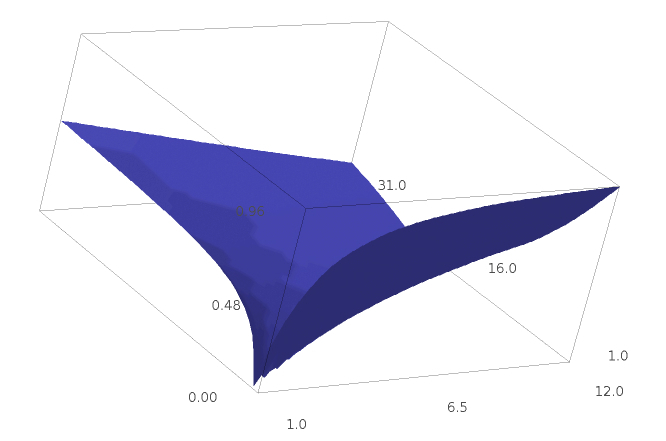
\includegraphics[height=2in]{gr/bin/rcbday.jpg}
          \end{center}
        \item Kita ingin memaksimumkan nilai berikut.
          \begin{equation*}
            \theta
            =
            \arccos(\,\frac{\colvec[r]{7 \\ 12}\dotprod\colvec{m \\ d}}{
                  \absval{\colvec[r]{7 \\ 12}\,}\cdot\absval{\colvec{m \\ d}\,} }\,)
          \end{equation*}
          Tentu saja, $m$ dan $d$ tidak dapat bernilai negatif sehingga kita
          tidak dapat memperoleh vektor yang ortogonal terhadap vektor yang
          diberikan.
          Skrip Python berikut menentukan sudut terbesar dengan pencarian
          menyeluruh.
\begin{lstlisting}
  import math
  days={1:31,  # Jan
        2:29, 3:31, 4:30, 5:31, 6:30, 7:31, 8:31, 9:30, 10:31, 11:30, 12:31}
  BDAY=(7,12)
  max_res=0
  max_res_date=(-1,-1)
  for month in range(1,13):
      for day in range(1,days[month]+1):
          num=BDAY[0]*month+BDAY[1]*day
          denom=math.sqrt(BDAY[0]**2+BDAY[1]**2)*math.sqrt(month**2+day**2)
          if denom>0:
              res=math.acos(min(num*1.0/denom,1))
              print("tanggal:",month,day," sudut:",res)
              if res>max_res:
                  max_res=res
                  max_res_date=(month,day)
  print("Untuk",BDAY,"kasus terburuk",max_res,"rad, tanggal",max_res_date)
  print("  Yaitu",180*max_res/math.pi,"derajat")
\end{lstlisting}
          Hasilnya adalah
\begin{lstlisting}
Untuk (7, 12) kasus terburuk 0.9595806464800957 rad, tanggal (12, 1)
  Yaitu 54.979921145744555 derajat
\end{lstlisting}

          Pendekatan yang lebih konseptual adalah meninjau hubungan semua titik
          $(\text{bulan},\text{tanggal})$ dengan titik $(7,12)$.
          Gambar berikut memperjelas bahwa jawabannya adalah $1$~Desember atau
          $31$~Januari, bergantung pada mana yang lebih jauh dari tanggal lahir
          tersebut.
          Garis putus-putus membagi dua sudut antara garis dari titik asal ke
          $1$~Desember dan garis dari titik asal ke $31$~Januari.
          Tanggal lahir di atas garis paling jauh dari $1$~Desember, sedangkan
          tanggal lahir di bawah garis paling jauh dari $31$~Januari.
          \begin{center}
            \includegraphics{gr/mp/ch1.54}
          \end{center}
      \end{exparts}
    \end{answer}
  \puzzle \item 
    \cite{Monthly33p118}
    Sebuah kapal berlayar dengan kecepatan dan arah \( \vec{v}_1 \); menurut
    penunjuk arah angin pada tiang, angin semu bertiup searah vektor
    \( \vec{a} \). Setelah arah dan kecepatan kapal diubah dari
    \( \vec{v}_1 \) menjadi \( \vec{v}_2 \), angin semu searah vektor
    \( \vec{b} \).

    Tentukan vektor kecepatan angin.
    \begin{answer}
      \answerasgiven %
      Kecepatan sebenarnya \( \vec{v} \) dari angin adalah jumlah kecepatan
      kapal dan kecepatan semu angin.
      Tanpa mengurangi keumuman, kita dapat menganggap \( \vec{a} \) dan
      \( \vec{b} \) sebagai vektor satuan dan menuliskan
      \begin{equation*}
         \vec{v}=\vec{v}_1+s\vec{a}=\vec{v}_2+t\vec{b}
      \end{equation*}
      dengan \( s \) dan \( t \) skalar yang belum ditentukan.
      Ambil hasil kali titiknya mula-mula dengan \( \vec{a} \), lalu dengan
      \( \vec{b} \), untuk memperoleh
      \begin{align*}
         s-t\vec{a}\dotprod\vec{b}
         &=\vec{a}\dotprod(\vec{v}_2-\vec{v}_1)    \\
         s\vec{a}\dotprod\vec{b}-t
         &=\vec{b}\dotprod(\vec{v}_2-\vec{v}_1)
      \end{align*}
      Kalikan persamaan kedua dengan \( \vec{a}\dotprod\vec{b} \),
      kurangkan hasilnya dari persamaan pertama, dan peroleh
      \begin{equation*}
         s=
         \frac{[\vec{a}-(\vec{a}\dotprod\vec{b})\vec{b}]
                   \dotprod(\vec{v}_2-\vec{v}_1)
              }{1-(\vec{a}\dotprod\vec{b})^2}.
      \end{equation*}
      Dengan menyubstitusikannya ke persamaan semula, kita memperoleh
      \begin{equation*}
         \vec{v}=\vec{v}_1+
         \frac{[\vec{a}-(\vec{a}\dotprod\vec{b})\vec{b}]
                  \dotprod(\vec{v}_2-\vec{v}_1)
              \vec{a}}{1-(\vec{a}\dotprod\vec{b})^2}.
      \end{equation*}
      Rumus ini berlaku jika \( \vec{a} \) dan \( \vec{b} \) tidak sejajar,
      sehingga penyebutnya tidak nol. Jika kedua arah semu sejajar, data yang
      diberikan tidak menentukan satu vektor kecepatan angin secara unik.
    \end{answer}
  \item  
     Buktikan ketaksamaan Cauchy--Schwarz dengan terlebih dahulu membuktikan
     identitas Lagrange:
     \begin{equation*}
      \left(\sum_{1\leq j\leq n} a_jb_j \right)^2
      =
      \left(\sum_{1\leq j\leq n}a_j^2\right)
      \left(\sum_{1\leq j\leq n}b_j^2\right)
      -
      \sum_{1\leq k < j\leq n}(a_kb_j-a_jb_k)^2
     \end{equation*}
     lalu perhatikan bahwa suku terakhir tidak negatif.
     % (Recall the meaning
     % \begin{equation*}
     %   \sum_{1\leq j\leq n}a_jb_j=
     %   a_1b_1+a_2b_2+\cdots+a_nb_n
     % \end{equation*}
     % and
     % \begin{equation*}
     %   \sum_{1\leq j\leq n}{a_j}^2=
     %   {a_1}^2+{a_2}^2+\cdots+{a_n}^2
     % \end{equation*}
     % of the \( \Sigma \) notation.)
     Hasil ini memperkuat Cauchy--Schwarz karena memberikan rumus untuk
     selisih antara kuadrat kedua ruas.
     Tafsirkan selisih kuadrat itu dalam \( \Re^2 \).
     \begin{answer}
       Kita menggunakan induksi pada \( n \).

       Pada kasus dasar \( n=1 \), identitas tersebut menjadi
       \begin{equation*}
          (a_1b_1)^2=({a_1}^2)({b_1}^2)-0
       \end{equation*}
       dan jelas berlaku.

       Untuk langkah induksi, andaikan rumus tersebut berlaku untuk kasus
       \( 1 \), \ldots, \( n \).
       Kita akan menunjukkan bahwa rumus itu juga berlaku untuk kasus
       \( n+1 \).
       Mulailah dari ruas kanan
       \begin{multline*}
         \bigl( \sum_{1\leq j\leq n+1}{a_j}^2\bigr)
         \bigl( \sum_{1\leq j\leq n+1}{b_j}^2\bigr)
         -
         \sum_{1\leq k<j\leq n+1}\bigl(a_kb_j-a_jb_k\bigr)^2  \\
       \begin{aligned}
         &=
         \bigl[ (\sum_{1\leq j\leq n}{a_j}^2)+{a_{n+1}}^2\bigr]
         \bigl[ (\sum_{1\leq j\leq n}{b_j}^2)+{b_{n+1}}^2\bigr]   \\     
         &\hbox{}\quad -
         \bigl[\sum_{1\leq k<j\leq n}\bigl(a_kb_j-a_jb_k\bigr)^2+
         \sum_{1\leq k\leq n}\bigl(a_kb_{n+1}-a_{n+1}b_k\bigr)^2  \bigr] \\
         &=
         \bigl( \sum_{1\leq j\leq n}{a_j}^2\bigr)
         \bigl( \sum_{1\leq j\leq n}{b_j}^2\bigr)
         +
         \sum_{1\leq j\leq n}{b_j}^2{a_{n+1}}^2                 
         +
         \sum_{1\leq j\leq n}{a_j}^2{b_{n+1}}^2
         +
         {a_{n+1}}^2{b_{n+1}}^2                                 \\
         &\hbox{}\qquad\hbox{} -
         \bigl[\sum_{1\leq k<j\leq n}\bigl(a_kb_j-a_jb_k\bigr)^2+
         \sum_{1\leq k\leq n}\bigl(a_kb_{n+1}-a_{n+1}b_k\bigr)^2  \bigr] \\
         &=
         \bigl( \sum_{1\leq j\leq n}{a_j}^2\bigr)
         \bigl( \sum_{1\leq j\leq n}{b_j}^2\bigr)
         -\sum_{1\leq k<j\leq n}\bigl(a_kb_j-a_jb_k\bigr)^2   \\   
         &\hbox{}\quad +
         \sum_{1\leq j\leq n}{b_j}^2{a_{n+1}}^2
         +
         \sum_{1\leq j\leq n}{a_j}^2{b_{n+1}}^2
         +
         {a_{n+1}}^2{b_{n+1}}^2                                 \\
         &\hbox{}\qquad\hbox{} -
         \sum_{1\leq k\leq n}\bigl(a_kb_{n+1}-a_{n+1}b_k\bigr)^2
        \end{aligned}
       \end{multline*}
       lalu terapkan hipotesis induksi.
       \begin{align*}
         &=
         \bigl( \sum_{1\leq j\leq n}a_jb_j\bigr)^2              
         +
         \sum_{1\leq j\leq n}{b_j}^2{a_{n+1}}^2
         +
         \sum_{1\leq j\leq n}{a_j}^2{b_{n+1}}^2
         +
         {a_{n+1}}^2{b_{n+1}}^2                          \\              
         &\hbox{}\qquad\hbox{}-
         \bigl[\sum_{1\leq k\leq n}{a_k}^2{b_{n+1}}^2
           -2\sum_{1\leq k\leq n}a_kb_{n+1}a_{n+1}b_k
           +\sum_{1\leq k\leq n}{a_{n+1}}^2{b_k}^2\bigr]        \\
         &=
         \bigl( \sum_{1\leq j\leq n}a_jb_j\bigr)^2
         +2\bigl(\sum_{1\leq k\leq n}a_kb_{n+1}a_{n+1}b_k\bigr)
         +{a_{n+1}}^2{b_{n+1}}^2                                 \\
         &=
         \bigl[\bigl(\sum_{1\leq j\leq n}a_jb_j\bigr)+a_{n+1}b_{n+1}\bigr]^2
       \end{align*}
       sehingga diperoleh ruas kiri.

       Dalam \( \Re^2 \), selisih antara kuadrat ruas kanan dan kuadrat ruas
       kiri Cauchy--Schwarz adalah
       \( (a_1b_2-a_2b_1)^2 \), yaitu kuadrat luas jajar genjang yang
       dibentang oleh \( (a_1,a_2) \) dan \( (b_1,b_2) \).
   \end{answer}
\end{exercises}
